%% Plantilla adaptada de la plantilla general LATEX para TFG de la UGR
%% Autor: Gabriel Maciá (gmacia@ugr.es)
%% Fecha: 14/06/2017


\documentclass[a4paper,11pt]{book}
%\documentclass[a4paper,twoside,11pt,titlepage]{book}
\usepackage{listings}
\usepackage[utf8]{inputenc}
\usepackage[spanish, es-tabla]{babel}

\decimalpoint
\usepackage{dcolumn}
\newcolumntype{.}{D{.}{\esperiod}{-1}}
\makeatletter
\addto\shorthandsspanish{\let\esperiod\es@period@code}
\makeatother
%\usepackage[chapter]{algorithm}
\RequirePackage{verbatim}
\usepackage{fancyhdr}
\usepackage{pdfpages}
\usepackage{graphicx}
\usepackage{epstopdf}
\usepackage{afterpage}
\usepackage{longtable}
\usepackage{hyperref} %referencia
\usepackage{bookmark}
	\bookmarksetup{numbered}
\usepackage{courier}
\usepackage{url}
\usepackage{colortbl,longtable}
\usepackage[stable]{footmisc}
\usepackage[acronym,nonumberlist]{glossaries}
	\setacronymstyle{long-short}
	\makeglossaries
	\renewcommand{\glossaryname}{Glosario de siglas}

\usepackage{dsfont}
%% Colocar aquí todas las palabras como queramos que se separen al terminar una línea. Ej. \hyphenation{co-mer}
\hyphenation{}


% Definición de comandos que me son tiles:
%\renewcommand{\indexname}{Índice alfabético}


\pagestyle{fancy}
\fancyhf{}
\fancyhead[LO]{\leftmark}
\fancyhead[RE]{\rightmark}
\fancyhead[RO,LE]{\textbf{\thepage}}
\renewcommand{\chaptermark}[1]{\markboth{\textbf{#1}}{}}
\renewcommand{\sectionmark}[1]{\markright{\textbf{\thesection. #1}}}
\setlength{\headheight}{1.5\headheight}
\newcommand{\HRule}{\rule{\linewidth}{0.5mm}}

%Definimos los tipos teorema, ejemplo y definición podremos usar estos tipos
%simplemente poniendo \begin{teorema} \end{teorema} ...
\newtheorem{teorema}{Teorema}[chapter]
\newtheorem{ejemplo}{Ejemplo}[chapter]
\newtheorem{definicion}{Definición}[chapter]

% Definiciones para listados de código

\definecolor{gray97}{gray}{.97}
\definecolor{gray75}{gray}{.75}
\definecolor{gray45}{gray}{.45}
\definecolor{gray30}{gray}{.94}
\definecolor{codegreen}{rgb}{0,0.6,0}
\definecolor{codegray}{rgb}{0.5,0.5,0.5}
\definecolor{codepurple}{rgb}{0.58,0,0.82}
\definecolor{backcolour}{rgb}{0.95,0.95,0.92}

\renewcommand\lstlistingname{Listado de código}
\renewcommand\lstlistlistingname{Listados de código}



\lstdefinestyle{Python}{
	backgroundcolor=\color{backcolour},   
	commentstyle=\color{codegreen},
	keywordstyle=\color{magenta},
	numberstyle=\tiny\color{codegray},
	stringstyle=\color{codepurple},
	basicstyle=\scriptsize\ttfamily,
	breakatwhitespace=false,         
	breaklines=true,                 
	captionpos=b,                    
	keepspaces=true,                 
	numbers=left,                    
	numbersep=5pt,                  
	showspaces=false,                
	showstringspaces=false,
	showtabs=false,                  
	tabsize=2
} 

\lstset{
    inputencoding=utf8,
    extendedchars=true,
    literate=%
    {á}{{\'a}}1
    {é}{{\'e}}1
    {í}{{\'i}}1
    {ñ}{{\~{n}}}1
    {ó}{{\'o}}1
    {ú}{{\'u}}1
    {Á}{{\'A}}1
    {É}{{\'E}}1
    {Í}{{\'I}}1
    {Ñ}{{\~{N}}}1
    {Ó}{{\'O}}1
    {Ú}{{\'U}}1
}
\usepackage{eurosym}

% minimizar fragmentado de listados
\lstnewenvironment{listing}[1][]
   {\lstset{#1}\pagebreak[0]}{\pagebreak[0]}

\lstset{style=Python}

%\lstdefinestyle{CodigoC}
%   {
%	basicstyle=\scriptsize,
%	frame=single,
%	language=C,
%	numbers=left
%   }
%\lstdefinestyle{CodigoC++}
%   {
%	basicstyle=\small,
%	frame=single,
%	backgroundcolor=\color{gray30},
%	language=C++,
%	numbers=left
%   }
%
%\lstdefinestyle{Consola}
%   {basicstyle=\scriptsize\bf\ttfamily,
%    backgroundcolor=\color{gray30},
%    frame=single,
%    numbers=none
%   }


\newcommand{\bigrule}{\titlerule[0.5mm]}

\DeclareMathOperator{\GF}{GF}


%Para conseguir que en las páginas en blanco no ponga cabecerass
\makeatletter
\def\clearpage{%
  \ifvmode
    \ifnum \@dbltopnum =\m@ne
      \ifdim \pagetotal <\topskip
        \hbox{}
      \fi
    \fi
  \fi
  \newpage
  \thispagestyle{empty}
  \write\m@ne{}
  \vbox{}
  \penalty -\@Mi
}
\makeatother

%TABLAS
\usepackage{tabularx}
\usepackage{float}
\usepackage{adjustbox}
\usepackage{booktabs}
\usepackage{multirow}
\usepackage{fourier} 
\usepackage{array}
\usepackage{makecell}

\renewcommand\theadalign{bc}
\renewcommand\theadfont{\bfseries}
\renewcommand\theadgape{\Gape[4pt]}
\renewcommand\cellgape{\Gape[4pt]}


%%%%%%%%%%%%%%%%%%%%%%%%%%%%%%%%%%%%%%%%%%%%%%%%%%%%%%%%%%%%%%%%%%%%%%%%%%%%%%%%%%%%%%%%
%% CONTENIDOS DEL DOCUMENTO
%%%%%%%%%%%%%%%%%%%%%%%%%%%%%%%%%%%%%%%%%%%%%%%%%%%%%%%%%%%%%%%%%%%%%%%%%%%%%%%%%%%%%%%%

\begin{document}


%\pdfbookmark[-1]{Memoria proyecto}{}
	\begin{titlepage}
 
 
\newlength{\centeroffset}
\setlength{\centeroffset}{-0.5\oddsidemargin}
\addtolength{\centeroffset}{0.5\evensidemargin}
\thispagestyle{empty}

\noindent\hspace*{\centeroffset}\begin{minipage}{\textwidth}

\centering
\includegraphics[width=0.9\textwidth]{portada/imagenes/logoModernoUGR.pdf}\\[1cm]

\textsc{ \Large TRABAJO FIN DE GRADO\\[0.2cm]}
\textsc{ DOBLE GRADO EN INGENIERÍA INFORMÁTICA Y MATEMÁTICAS }\\[1cm]
% Upper part of the page
% 
% Title
{\Huge\bfseries Implementación de una blockchain resistente a ataques criptográficos cuánticos\\
}
\end{minipage}

\vspace{1.3cm}
\noindent\hspace*{\centeroffset}\begin{minipage}{\textwidth}
\centering

\textbf{Autor}\\ {María Victoria Granados Pozo}\\[2.5ex]
\textbf{Directores}\\
{Gabriel Maciá Fernández\\
Francisco Javier Lobillo Borrero 
}\\[1.8cm]

%\nonindent
\includegraphics[width=0.3\textwidth]{portada/imagenes/logoEtsiit.pdf} \hfill \hfill \includegraphics[width=0.20\textwidth]{portada/imagenes/logoCiencias.png}\\[0.1cm]
\hbox{
	\vbox{
	  \hbox{\textsc{Escuela Técnica Superior de Ingenierías}}
	  \hbox{\textsc{Informática y de Telecomunicación}}
	}
	\hspace{1.6cm}
	\textsc{Facultad de Ciencias}
}

\vspace{1.4cm}

\textsc{---}\\
Granada, 18 de noviembre de 2020
\end{minipage}
%\addtolength{\textwidth}{\centeroffset}
%\vspace{\stretch{2}}
\end{titlepage}



	\chapter*{}
%\thispagestyle{empty}
%\cleardoublepage

%\thispagestyle{empty}

\begin{titlepage}
 
 
\setlength{\centeroffset}{-0.5\oddsidemargin}
\addtolength{\centeroffset}{0.5\evensidemargin}
\thispagestyle{empty}

\noindent\hspace*{\centeroffset}\begin{minipage}{\textwidth}

\centering
%\includegraphics[width=0.9\textwidth]{imagenes/logo_ugr.jpg}\\[1.4cm]

%\textsc{ \Large PROYECTO FIN DE CARRERA\\[0.2cm]}
%\textsc{ INGENIERÍA EN INFORMÁTICA}\\[1cm]
% Upper part of the page
% 

 \vspace{3.3cm}

%si el proyecto tiene logo poner aquí
%\includegraphics{portada/imagenes/logo.png} 
% \vspace{0.5cm}

% Title

{\Huge\bfseries Implementación de una blockchain resistente a ataques criptográficos cuánticos\\
}
\noindent\rule[-1ex]{\textwidth}{3pt}\\[3.5ex]
{\large\bfseries Subtítulo del proyecto.\\[4cm]}
\end{minipage}

\vspace{2.5cm}
\noindent\hspace*{\centeroffset}\begin{minipage}{\textwidth}
\centering

\textbf{Autor}\\ {María Victoria Granados Pozo}\\[2.5ex]
\textbf{Director}\\
{Gabriel Maciá Fernández\\
Francisco Javier Lobillo Borrero 
}\\[2cm]
%\includegraphics[width=0.15\textwidth]{imagenes/tstc.png}\\[0.1cm]
%\textsc{Departamento de Teoría de la Señal, Telemática y Comunicaciones}\\
%\textsc{---}\\
Granada, 18 de noviembre de 2020
\end{minipage}
%\addtolength{\textwidth}{\centeroffset}
\vspace{\stretch{2}}

 
\end{titlepage}






\cleardoublepage
\thispagestyle{empty}

\begin{center}
{\large\bfseries Implementación de una blockchain resistente a ataques criptográficos cuánticos}\\
\end{center}
\begin{center}
María Victoria Granados Pozo\\
\end{center}

%\vspace{0.7cm}
\noindent{\textbf{Palabras clave}: palabra\_clave1, palabra\_clave2, palabra\_clave3, ......}\\

\vspace{0.7cm}
\noindent{\textbf{Resumen}}\\

Poner aquí el resumen.
\cleardoublepage


\thispagestyle{empty}


\begin{center}
{\large\bfseries Implementation of a blockchain resistant to quantum cryptographic attacks}\\
\end{center}
\begin{center}
María Victoria Granados Pozo\\
\end{center}

%\vspace{0.7cm}
\noindent{\textbf{Keywords}: Keyword1, Keyword2, Keyword3, ....}\\

\vspace{0.7cm}
\noindent{\textbf{Abstract}}\\

Write here the abstract in English.

\chapter*{}
\thispagestyle{empty}

\noindent\rule[-1ex]{\textwidth}{2pt}\\[4.5ex]

Yo, \textbf{María Victoria Granados Pozo}, alumno de la titulación Doble Grado de Ingeniería Informática y Matemáticas de la \textbf{Escuela Técnica Superior
de Ingenierías Informática y de Telecomunicación y Facultad de Ciencias de la Universidad de Granada}, con DNI 77137043, autorizo la
ubicación de la siguiente copia de mi Trabajo Fin de Grado en la biblioteca del centro para que pueda ser
consultada por las personas que lo deseen.

\vspace{6cm}

\noindent Fdo: María Victoria Granados Pozo

\vspace{2cm}

\begin{flushright}
Granada a 18 de noviembre de 2020 .
\end{flushright}


\chapter*{}
\thispagestyle{empty}

\noindent\rule[-1ex]{\textwidth}{2pt}\\[4.5ex]

D. \textbf{Gabriel Maciá Fernández}, Profesor del Área de Ingeniería Telemática del Departamento de Teoría de la Señal, Telemática y Comunicaciones de la Universidad de Granada.

\vspace{0.5cm}

D. \textbf{Francisco Javier Lobillo Borrero}, Profesor del Área de Matemáticas del Departamento Álgebra de la Universidad de Granada.


\vspace{0.5cm}

\textbf{Informan:}

\vspace{0.5cm}

Que el presente trabajo, titulado \textit{\textbf{ Implementación de una blockchain resistente a ataques criptográficos cuánticos}},
ha sido realizado bajo su supervisión por \textbf{María Victoria Granados Pozo}, y autoriza la defensa de dicho trabajo ante el tribunal
que corresponda.

\vspace{0.5cm}

Y para que conste, expide y firma el presente informe en Granada a 18 de noviembre de 2020 .

\vspace{1cm}

\textbf{Los directores:}

\vspace{5cm}

\noindent \textbf{Gabriel Maciá Fernández \ \ \ \ \ Francisco Javier Lobillo Borrero}

\chapter*{Agradecimientos}
\thispagestyle{empty}

       \vspace{1cm}


En especial agradezco a mis tutores Grabiel Maciá y Javier Lobillo, por el apoyo y la paciencia que han tenido conmigo a lo largos de todos estos meses. También a Javier Tallón por orientarme a elegir el tema de este trabajo.\\

A mis padres, Miguel y Esther, que me han soportado y animado en los momentos más difíciles. A mi hermano, Miguel, por darme fuerza en el día a día en estos momentos tan complicados de la pandemia que nos ha tocado vivir.\\

Por último, agradecer a los profesores y compañeros que me he encontrado a lo largo de estos cinco años de carrera, que tanto me han enseñado y tantos momentos he compartido con ellos.\\








	\frontmatter
	\pdfbookmark[0]{Índice}{}
	\tableofcontents
	\listoffigures
	\listoftables
	\lstlistoflistings
	\mainmatter

% Ficheros con los contenidos

	%

\chapter*{Guía de estilo para escribir un TFG/TFM} \addcontentsline{toc}{chapter}{Guía de estilo}

Este capítulo no forma parte del TFG/TFM. Su único objetivo es aportar algunas recomendaciones y plantillas para tener claro cómo redactar el TFG/TFM. Una vez se haya comprendido, se puede comentar la siguiente línea en el fichero proyecto.tex añadiéndole al principio el carácter \%: 
\begin{verbatim}


\chapter*{Guía de estilo para escribir un TFG/TFM} \addcontentsline{toc}{chapter}{Guía de estilo}

Este capítulo no forma parte del TFG/TFM. Su único objetivo es aportar algunas recomendaciones y plantillas para tener claro cómo redactar el TFG/TFM. Una vez se haya comprendido, se puede comentar la siguiente línea en el fichero proyecto.tex añadiéndole al principio el carácter \%: 
\begin{verbatim}


\chapter*{Guía de estilo para escribir un TFG/TFM} \addcontentsline{toc}{chapter}{Guía de estilo}

Este capítulo no forma parte del TFG/TFM. Su único objetivo es aportar algunas recomendaciones y plantillas para tener claro cómo redactar el TFG/TFM. Una vez se haya comprendido, se puede comentar la siguiente línea en el fichero proyecto.tex añadiéndole al principio el carácter \%: 
\begin{verbatim}
\input{guiaDeEstilo} --> %\input{guiaDeEstilo}
\end{verbatim}

\section*{Recomendaciones generales}
A la hora de escribir el TFG/TFM es importante seguir las siguientes recomendaciones: 

\begin{enumerate}
	\item La memoria debe realizarse con el \textbf{máximo cuidado}, y debe proporcionar de forma consistente -y por sí misma- una idea clara y concisa de lo que se ha realizado. 
	\item No debe tener errores tipográficos ni ortográficos. Este es un aspecto que penaliza muchísimo el trabajo en la evaluación del tribunal. 
	\item Siempre que se utilice alguna figura no elaborada por el autor del proyecto debe indicarse la fuente de la que se ha sacado mediante una cita en la bibliografía. 
	\item La lectura debe ser fluida. Por ello, dada la dificultad que tiene afrontar la escritura de un texto largo casi por primera vez, se recomienda elaborar un índice rellenando los títulos de los diferentes apartados de que constará este documento. En segundo lugar, para cada apartado, se indicarán a modo de resumen las diferentes ideas que se desarrollarán posteriormente (una línea de texto por idea). Después, se desarrollan las ideas (cada idea en un párrafo). Cuando se termina, se realiza una lectura completa y detallada del texto para comprobar que es coherente y no tiene fallos ortográficos, tipográficos ni gramaticales, antes de pasarlo al tutor. 
	\item Una extensión normal está entorno a las 100-120 páginas. Esto no quiere decir que tengamos que escribir por escribir, ni meter contenido adicional sin sentido. Hay que escribir el proyecto de forma coherente, pero sin ser telegráfico, esto es, realizando una descripción detallada del trabajo realizado. 
	\item Evitar afirmaciones del tipo “El sistema diseñado es bastante bueno”. Esa misma frase debería ser escrita tal que responda a las preguntas: ¿Qué parte del sistema? ¿En qué sentido? ¿Cuánto de bueno? ¿Comparado con qué?
	\item Evitar la primera persona (incluso del plural). No obstante para resaltar la autoría de algo o enfatizar una posición personal sí se puede usar.
	\item Numerar estructuradamente los capítulos, secciones y subsecciones. Evitar más de tres niveles de anidamiento. 
	\item Toda afirmación categórica o se demuestra (teórica o experimentalmente)  o se incluye una referencia en la que se haya previamente demostrado.
	\item Toda tecnología, teorema, institución, norma, documento que se mencione debe estar referenciado. No incluir referencias a la wiki.
	\item Los términos en ingles que no tenga sentido traducir se pondrán en cursiva al menos para indicar que es un término no castellano.
	 

\end{enumerate}

\section*{Recomendaciones específicas para determinados contenidos}

\subsection*{Inserción de figuras}
Esta es una plantilla de código para adjuntar una figura. 

% El verbatim es solo para poner en el PDF el código que corresponde a la inserción de la figura
\begin{verbatim}
\begin{figure}[t]
	\centering
		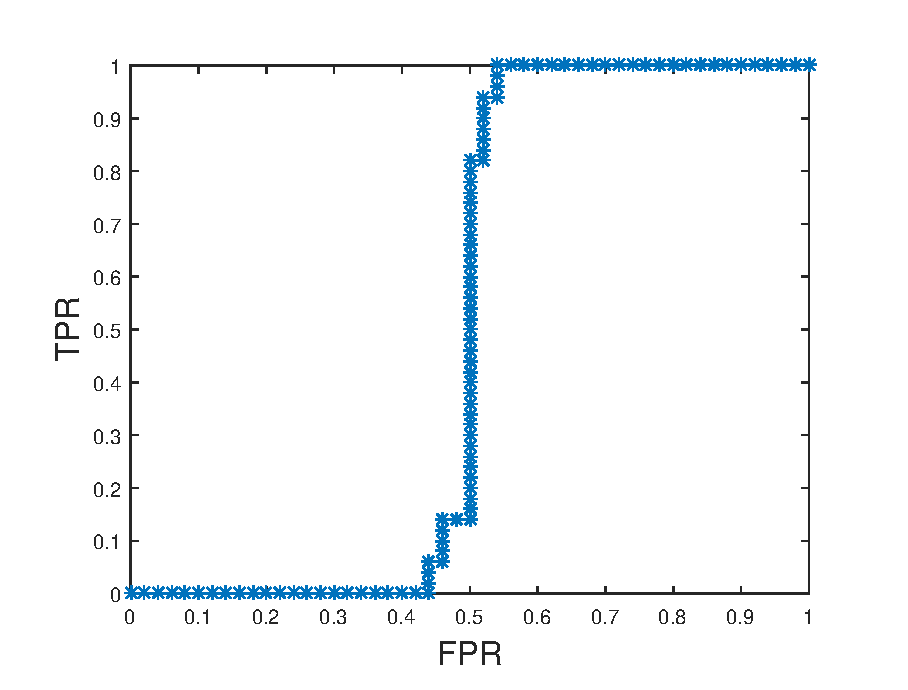
\includegraphics[width=0.6\textwidth]{figuras/prueba.eps}
	\caption{Pie de figura. Poner aquí cita del lugar de donde 
	se ha tomado la imagen en caso de que sea así. }
	\label{fig:prueba}
\end{figure}
\end{verbatim}

% Y ahora pongo la plantilla para que se incluya la figura efectivamente
\begin{figure}[t]
	\centering
	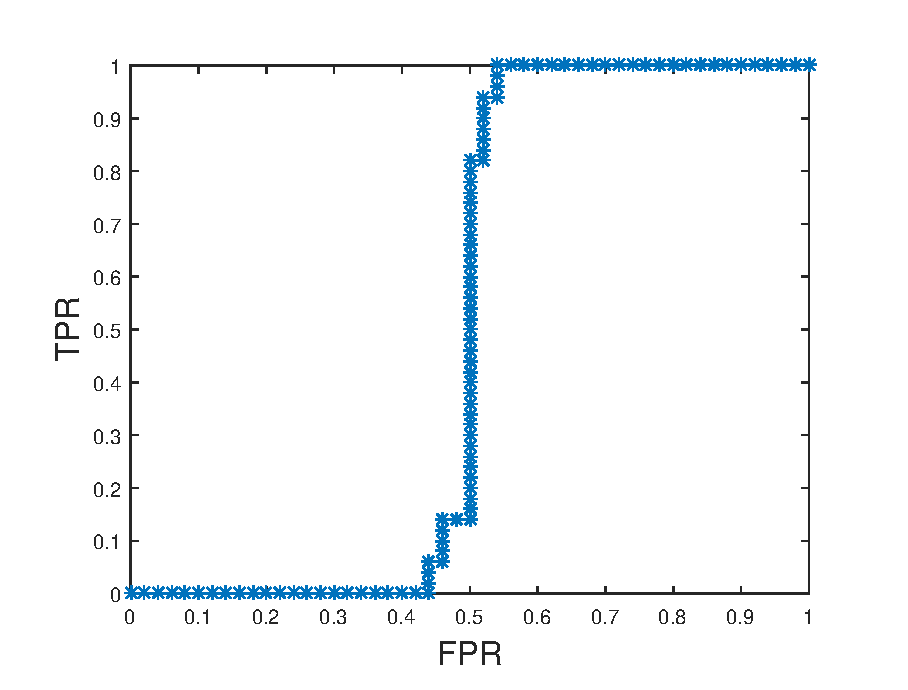
\includegraphics[width=0.6\textwidth]{figuras/prueba.eps}
	\caption{Pie de figura. Poner aquí cita del lugar de donde se ha tomado la imagen en caso de que sea así. }
	\label{fig:prueba}
\end{figure}

Si se pone el modificador [t] (top) latex ubicará la figura en la parte de arriba de la página. Ver otros modificadores como [h] (here) o [b] (bottom). Se pueden usar otras plantillas para, por ejemplo, poner dos figuras una al lado de otra. Consultar en Internet diferentes plantillas en caso de necesidad. 

Cuando en el texto nos refiramos a la figura en cuestión por el número, debemos usar la mayúscula y utilizar referencia a la figura. Esto hará que no nos tengamos que preocupar de la numeración de las figuras. Ej. Como se puede comprobar en la Figura~\ref{fig:prueba}.

Sustituir expresiones del tipo: “En la siguiente figura…” por “En la Figura 2.2…”


\subsection*{Inserción de tablas}

Este sería un ejemplo de una tabla. Se puede modificar el formato y contenido (ver en Internet algún enlace sobre cómo formatear tablas en latex). 

\begin{table}[t]
	\caption{Descripción de la tabla.}
	\label{table:prueba}
	\centering
	\begin{tabular}{l  c} 
		\hline \\[-1.5ex]
		\textbf{Tipo de ataque} & \textbf{Etiqueta} \\ [1ex] 
		\hline\hline \\[-1.5ex]
		DoS11 & dos \\ [0.5ex]
		Exf1MBp & exf1KB \\ [1ex]
		\hline
	\end{tabular}
\end{table}

La forma de referirse a las tablas es similar a las de las figuras (usar mayúsculas y referencia a la etiqueta(label) de la tabla). Ej. Como se puede ver en la Tabla~\ref{table:prueba}, ...


\subsection*{Citas de bibliografía}
Ejemplo de cita de bibliografía. Primero se va a google.scholar y se busca la referencia. Después se da al enlace citar, y se elige el formato bibtex. Se copia ese texto en el fichero bibliografia.bib. Un ejemplo de referenciar una cita es \cite{macia2008evaluation}.


\subsection*{Referencias a secciones}

Para referirnos a secciones, primero debemos tener una etiqueta de tipo \texttt{label} en dicha sección. Posteriormente, pondremos una referencia a dicho label, igual que hacemos para las figuras y las tablas. Ej. Como se ha mencionado en la Sección~\ref{sec:intro:motivacion} (Nótese que la palabra Sección va con mayúscula).

\subsection*{Glosario y acrónimos}

Cuando se utilice un acrónimo se debe definir en el fichero glosario/entradas\_glosario, tal y como está el ejemplo en dicho fichero. Al referirse en el texto se indicará así: \gls{svm} (ver que la primera vez lo pondrá completo). La segunda vez que se referencie a \gls{svm} ya no aparece completo. También se puede nombrar en plural así: \glspl{svm}. 
Otros ejemplos de acrónimo son: \gls{gcd}, \gls{lcm}, \gls{gmf}. 

A la hora de compilar con el glosario, se debe abrir una terminal CMD en el directorio de los fuentes latex del proyecto, y ejecutar el siguiente comando: \texttt{makeglossaries proyecto}. Esto generará los ficheros auxiliares que contienen el glosario. 

\subsection*{Listados de código}

Aquí se puede ver un ejemplo de listado de código: 

%\begin{lstlisting}[frame=none, numbers=none]


\begin{lstlisting}[language=Python,caption=Ejemplo de Python, label=listado:pythonPrueba]
import numpy as np

def incmatrix(genl1,genl2):
	m = len(genl1)
	n = len(genl2)
	M = None #to become the incidence matrix
	VT = np.zeros((n*m,1), int)  #dummy variable

	#compute the bitwise xor matrix
	M1 = bitxormatrix(genl1)
	M2 = np.triu(bitxormatrix(genl2),1) 
	
	for i in range(m-1):
		for j in range(i+1, m):
			[r,c] = np.where(M2 == M1[i,j])
			for k in range(len(r)):
				VT[(i)*n + r[k]] = 1;
				VT[(i)*n + c[k]] = 1;
				VT[(j)*n + r[k]] = 1;
				VT[(j)*n + c[k]] = 1;
	
	if M is None:
		M = np.copy(VT)
	else:
		M = np.concatenate((M, VT), 1)
	
	VT = np.zeros((n*m,1), int)
	
	return M

\end{lstlisting}

Nos podemos referir a él como Listado de código~\ref{listado:pythonPrueba}. 
Si queremos que aparezca como un flotante en la página debemos poner la palabra \texttt{float} así: 
\begin{verbatim}
\begin{lstlisting}[float,language=Python,caption=Ejemplo de Python, 
label=listado:pythonPrueba]
\end{verbatim}


\subsection*{Enlaces URL}
Podemos poner un enlace así \url{http://dtstc.ugr.es/~gmacia} --> %

\chapter*{Guía de estilo para escribir un TFG/TFM} \addcontentsline{toc}{chapter}{Guía de estilo}

Este capítulo no forma parte del TFG/TFM. Su único objetivo es aportar algunas recomendaciones y plantillas para tener claro cómo redactar el TFG/TFM. Una vez se haya comprendido, se puede comentar la siguiente línea en el fichero proyecto.tex añadiéndole al principio el carácter \%: 
\begin{verbatim}
\input{guiaDeEstilo} --> %\input{guiaDeEstilo}
\end{verbatim}

\section*{Recomendaciones generales}
A la hora de escribir el TFG/TFM es importante seguir las siguientes recomendaciones: 

\begin{enumerate}
	\item La memoria debe realizarse con el \textbf{máximo cuidado}, y debe proporcionar de forma consistente -y por sí misma- una idea clara y concisa de lo que se ha realizado. 
	\item No debe tener errores tipográficos ni ortográficos. Este es un aspecto que penaliza muchísimo el trabajo en la evaluación del tribunal. 
	\item Siempre que se utilice alguna figura no elaborada por el autor del proyecto debe indicarse la fuente de la que se ha sacado mediante una cita en la bibliografía. 
	\item La lectura debe ser fluida. Por ello, dada la dificultad que tiene afrontar la escritura de un texto largo casi por primera vez, se recomienda elaborar un índice rellenando los títulos de los diferentes apartados de que constará este documento. En segundo lugar, para cada apartado, se indicarán a modo de resumen las diferentes ideas que se desarrollarán posteriormente (una línea de texto por idea). Después, se desarrollan las ideas (cada idea en un párrafo). Cuando se termina, se realiza una lectura completa y detallada del texto para comprobar que es coherente y no tiene fallos ortográficos, tipográficos ni gramaticales, antes de pasarlo al tutor. 
	\item Una extensión normal está entorno a las 100-120 páginas. Esto no quiere decir que tengamos que escribir por escribir, ni meter contenido adicional sin sentido. Hay que escribir el proyecto de forma coherente, pero sin ser telegráfico, esto es, realizando una descripción detallada del trabajo realizado. 
	\item Evitar afirmaciones del tipo “El sistema diseñado es bastante bueno”. Esa misma frase debería ser escrita tal que responda a las preguntas: ¿Qué parte del sistema? ¿En qué sentido? ¿Cuánto de bueno? ¿Comparado con qué?
	\item Evitar la primera persona (incluso del plural). No obstante para resaltar la autoría de algo o enfatizar una posición personal sí se puede usar.
	\item Numerar estructuradamente los capítulos, secciones y subsecciones. Evitar más de tres niveles de anidamiento. 
	\item Toda afirmación categórica o se demuestra (teórica o experimentalmente)  o se incluye una referencia en la que se haya previamente demostrado.
	\item Toda tecnología, teorema, institución, norma, documento que se mencione debe estar referenciado. No incluir referencias a la wiki.
	\item Los términos en ingles que no tenga sentido traducir se pondrán en cursiva al menos para indicar que es un término no castellano.
	 

\end{enumerate}

\section*{Recomendaciones específicas para determinados contenidos}

\subsection*{Inserción de figuras}
Esta es una plantilla de código para adjuntar una figura. 

% El verbatim es solo para poner en el PDF el código que corresponde a la inserción de la figura
\begin{verbatim}
\begin{figure}[t]
	\centering
		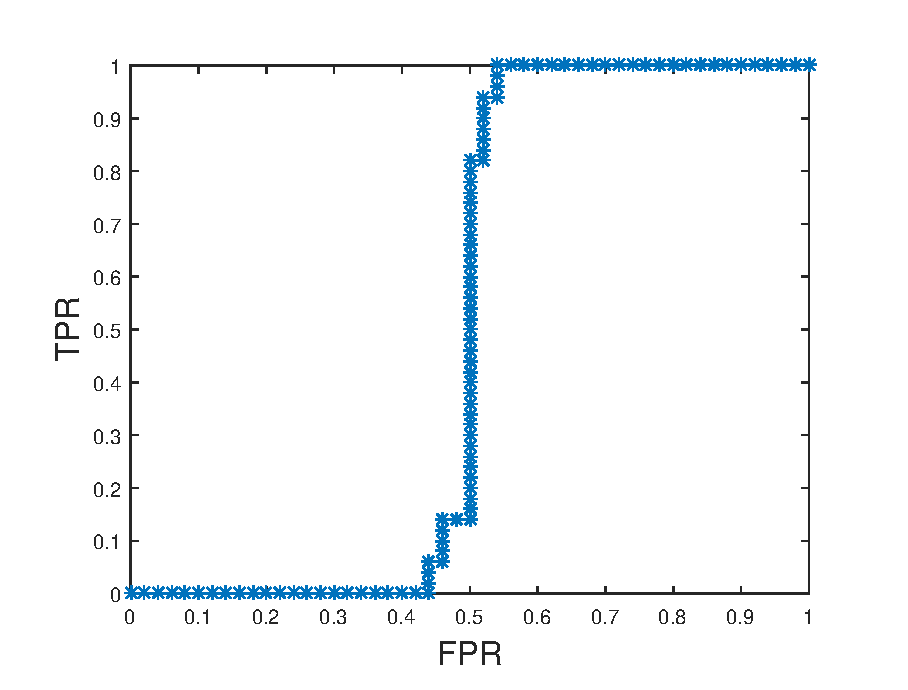
\includegraphics[width=0.6\textwidth]{figuras/prueba.eps}
	\caption{Pie de figura. Poner aquí cita del lugar de donde 
	se ha tomado la imagen en caso de que sea así. }
	\label{fig:prueba}
\end{figure}
\end{verbatim}

% Y ahora pongo la plantilla para que se incluya la figura efectivamente
\begin{figure}[t]
	\centering
	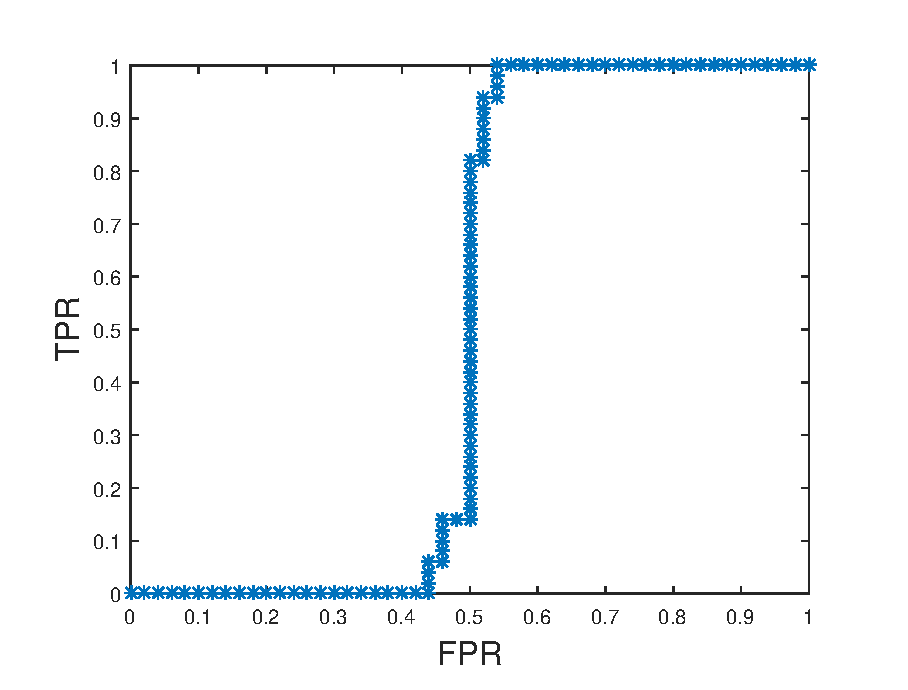
\includegraphics[width=0.6\textwidth]{figuras/prueba.eps}
	\caption{Pie de figura. Poner aquí cita del lugar de donde se ha tomado la imagen en caso de que sea así. }
	\label{fig:prueba}
\end{figure}

Si se pone el modificador [t] (top) latex ubicará la figura en la parte de arriba de la página. Ver otros modificadores como [h] (here) o [b] (bottom). Se pueden usar otras plantillas para, por ejemplo, poner dos figuras una al lado de otra. Consultar en Internet diferentes plantillas en caso de necesidad. 

Cuando en el texto nos refiramos a la figura en cuestión por el número, debemos usar la mayúscula y utilizar referencia a la figura. Esto hará que no nos tengamos que preocupar de la numeración de las figuras. Ej. Como se puede comprobar en la Figura~\ref{fig:prueba}.

Sustituir expresiones del tipo: “En la siguiente figura…” por “En la Figura 2.2…”


\subsection*{Inserción de tablas}

Este sería un ejemplo de una tabla. Se puede modificar el formato y contenido (ver en Internet algún enlace sobre cómo formatear tablas en latex). 

\begin{table}[t]
	\caption{Descripción de la tabla.}
	\label{table:prueba}
	\centering
	\begin{tabular}{l  c} 
		\hline \\[-1.5ex]
		\textbf{Tipo de ataque} & \textbf{Etiqueta} \\ [1ex] 
		\hline\hline \\[-1.5ex]
		DoS11 & dos \\ [0.5ex]
		Exf1MBp & exf1KB \\ [1ex]
		\hline
	\end{tabular}
\end{table}

La forma de referirse a las tablas es similar a las de las figuras (usar mayúsculas y referencia a la etiqueta(label) de la tabla). Ej. Como se puede ver en la Tabla~\ref{table:prueba}, ...


\subsection*{Citas de bibliografía}
Ejemplo de cita de bibliografía. Primero se va a google.scholar y se busca la referencia. Después se da al enlace citar, y se elige el formato bibtex. Se copia ese texto en el fichero bibliografia.bib. Un ejemplo de referenciar una cita es \cite{macia2008evaluation}.


\subsection*{Referencias a secciones}

Para referirnos a secciones, primero debemos tener una etiqueta de tipo \texttt{label} en dicha sección. Posteriormente, pondremos una referencia a dicho label, igual que hacemos para las figuras y las tablas. Ej. Como se ha mencionado en la Sección~\ref{sec:intro:motivacion} (Nótese que la palabra Sección va con mayúscula).

\subsection*{Glosario y acrónimos}

Cuando se utilice un acrónimo se debe definir en el fichero glosario/entradas\_glosario, tal y como está el ejemplo en dicho fichero. Al referirse en el texto se indicará así: \gls{svm} (ver que la primera vez lo pondrá completo). La segunda vez que se referencie a \gls{svm} ya no aparece completo. También se puede nombrar en plural así: \glspl{svm}. 
Otros ejemplos de acrónimo son: \gls{gcd}, \gls{lcm}, \gls{gmf}. 

A la hora de compilar con el glosario, se debe abrir una terminal CMD en el directorio de los fuentes latex del proyecto, y ejecutar el siguiente comando: \texttt{makeglossaries proyecto}. Esto generará los ficheros auxiliares que contienen el glosario. 

\subsection*{Listados de código}

Aquí se puede ver un ejemplo de listado de código: 

%\begin{lstlisting}[frame=none, numbers=none]


\begin{lstlisting}[language=Python,caption=Ejemplo de Python, label=listado:pythonPrueba]
import numpy as np

def incmatrix(genl1,genl2):
	m = len(genl1)
	n = len(genl2)
	M = None #to become the incidence matrix
	VT = np.zeros((n*m,1), int)  #dummy variable

	#compute the bitwise xor matrix
	M1 = bitxormatrix(genl1)
	M2 = np.triu(bitxormatrix(genl2),1) 
	
	for i in range(m-1):
		for j in range(i+1, m):
			[r,c] = np.where(M2 == M1[i,j])
			for k in range(len(r)):
				VT[(i)*n + r[k]] = 1;
				VT[(i)*n + c[k]] = 1;
				VT[(j)*n + r[k]] = 1;
				VT[(j)*n + c[k]] = 1;
	
	if M is None:
		M = np.copy(VT)
	else:
		M = np.concatenate((M, VT), 1)
	
	VT = np.zeros((n*m,1), int)
	
	return M

\end{lstlisting}

Nos podemos referir a él como Listado de código~\ref{listado:pythonPrueba}. 
Si queremos que aparezca como un flotante en la página debemos poner la palabra \texttt{float} así: 
\begin{verbatim}
\begin{lstlisting}[float,language=Python,caption=Ejemplo de Python, 
label=listado:pythonPrueba]
\end{verbatim}


\subsection*{Enlaces URL}
Podemos poner un enlace así \url{http://dtstc.ugr.es/~gmacia}
\end{verbatim}

\section*{Recomendaciones generales}
A la hora de escribir el TFG/TFM es importante seguir las siguientes recomendaciones: 

\begin{enumerate}
	\item La memoria debe realizarse con el \textbf{máximo cuidado}, y debe proporcionar de forma consistente -y por sí misma- una idea clara y concisa de lo que se ha realizado. 
	\item No debe tener errores tipográficos ni ortográficos. Este es un aspecto que penaliza muchísimo el trabajo en la evaluación del tribunal. 
	\item Siempre que se utilice alguna figura no elaborada por el autor del proyecto debe indicarse la fuente de la que se ha sacado mediante una cita en la bibliografía. 
	\item La lectura debe ser fluida. Por ello, dada la dificultad que tiene afrontar la escritura de un texto largo casi por primera vez, se recomienda elaborar un índice rellenando los títulos de los diferentes apartados de que constará este documento. En segundo lugar, para cada apartado, se indicarán a modo de resumen las diferentes ideas que se desarrollarán posteriormente (una línea de texto por idea). Después, se desarrollan las ideas (cada idea en un párrafo). Cuando se termina, se realiza una lectura completa y detallada del texto para comprobar que es coherente y no tiene fallos ortográficos, tipográficos ni gramaticales, antes de pasarlo al tutor. 
	\item Una extensión normal está entorno a las 100-120 páginas. Esto no quiere decir que tengamos que escribir por escribir, ni meter contenido adicional sin sentido. Hay que escribir el proyecto de forma coherente, pero sin ser telegráfico, esto es, realizando una descripción detallada del trabajo realizado. 
	\item Evitar afirmaciones del tipo “El sistema diseñado es bastante bueno”. Esa misma frase debería ser escrita tal que responda a las preguntas: ¿Qué parte del sistema? ¿En qué sentido? ¿Cuánto de bueno? ¿Comparado con qué?
	\item Evitar la primera persona (incluso del plural). No obstante para resaltar la autoría de algo o enfatizar una posición personal sí se puede usar.
	\item Numerar estructuradamente los capítulos, secciones y subsecciones. Evitar más de tres niveles de anidamiento. 
	\item Toda afirmación categórica o se demuestra (teórica o experimentalmente)  o se incluye una referencia en la que se haya previamente demostrado.
	\item Toda tecnología, teorema, institución, norma, documento que se mencione debe estar referenciado. No incluir referencias a la wiki.
	\item Los términos en ingles que no tenga sentido traducir se pondrán en cursiva al menos para indicar que es un término no castellano.
	 

\end{enumerate}

\section*{Recomendaciones específicas para determinados contenidos}

\subsection*{Inserción de figuras}
Esta es una plantilla de código para adjuntar una figura. 

% El verbatim es solo para poner en el PDF el código que corresponde a la inserción de la figura
\begin{verbatim}
\begin{figure}[t]
	\centering
		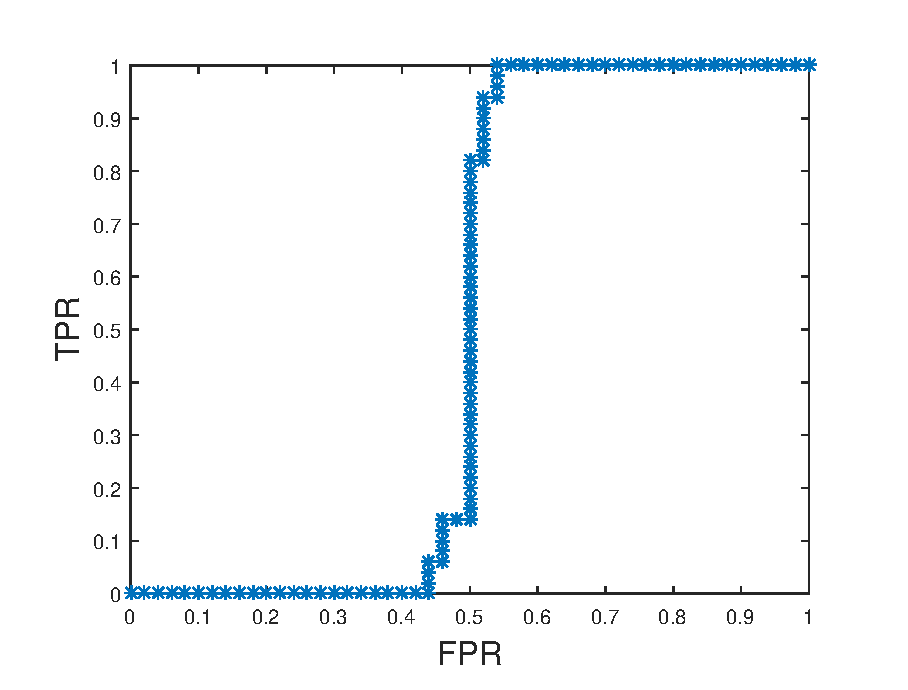
\includegraphics[width=0.6\textwidth]{figuras/prueba.eps}
	\caption{Pie de figura. Poner aquí cita del lugar de donde 
	se ha tomado la imagen en caso de que sea así. }
	\label{fig:prueba}
\end{figure}
\end{verbatim}

% Y ahora pongo la plantilla para que se incluya la figura efectivamente
\begin{figure}[t]
	\centering
	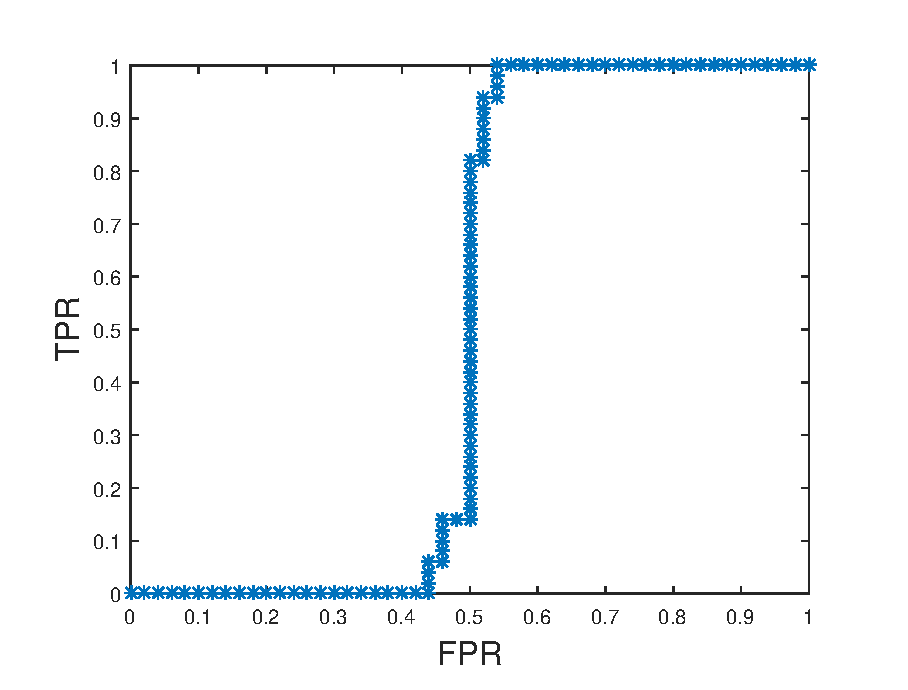
\includegraphics[width=0.6\textwidth]{figuras/prueba.eps}
	\caption{Pie de figura. Poner aquí cita del lugar de donde se ha tomado la imagen en caso de que sea así. }
	\label{fig:prueba}
\end{figure}

Si se pone el modificador [t] (top) latex ubicará la figura en la parte de arriba de la página. Ver otros modificadores como [h] (here) o [b] (bottom). Se pueden usar otras plantillas para, por ejemplo, poner dos figuras una al lado de otra. Consultar en Internet diferentes plantillas en caso de necesidad. 

Cuando en el texto nos refiramos a la figura en cuestión por el número, debemos usar la mayúscula y utilizar referencia a la figura. Esto hará que no nos tengamos que preocupar de la numeración de las figuras. Ej. Como se puede comprobar en la Figura~\ref{fig:prueba}.

Sustituir expresiones del tipo: “En la siguiente figura…” por “En la Figura 2.2…”


\subsection*{Inserción de tablas}

Este sería un ejemplo de una tabla. Se puede modificar el formato y contenido (ver en Internet algún enlace sobre cómo formatear tablas en latex). 

\begin{table}[t]
	\caption{Descripción de la tabla.}
	\label{table:prueba}
	\centering
	\begin{tabular}{l  c} 
		\hline \\[-1.5ex]
		\textbf{Tipo de ataque} & \textbf{Etiqueta} \\ [1ex] 
		\hline\hline \\[-1.5ex]
		DoS11 & dos \\ [0.5ex]
		Exf1MBp & exf1KB \\ [1ex]
		\hline
	\end{tabular}
\end{table}

La forma de referirse a las tablas es similar a las de las figuras (usar mayúsculas y referencia a la etiqueta(label) de la tabla). Ej. Como se puede ver en la Tabla~\ref{table:prueba}, ...


\subsection*{Citas de bibliografía}
Ejemplo de cita de bibliografía. Primero se va a google.scholar y se busca la referencia. Después se da al enlace citar, y se elige el formato bibtex. Se copia ese texto en el fichero bibliografia.bib. Un ejemplo de referenciar una cita es \cite{macia2008evaluation}.


\subsection*{Referencias a secciones}

Para referirnos a secciones, primero debemos tener una etiqueta de tipo \texttt{label} en dicha sección. Posteriormente, pondremos una referencia a dicho label, igual que hacemos para las figuras y las tablas. Ej. Como se ha mencionado en la Sección~\ref{sec:intro:motivacion} (Nótese que la palabra Sección va con mayúscula).

\subsection*{Glosario y acrónimos}

Cuando se utilice un acrónimo se debe definir en el fichero glosario/entradas\_glosario, tal y como está el ejemplo en dicho fichero. Al referirse en el texto se indicará así: \gls{svm} (ver que la primera vez lo pondrá completo). La segunda vez que se referencie a \gls{svm} ya no aparece completo. También se puede nombrar en plural así: \glspl{svm}. 
Otros ejemplos de acrónimo son: \gls{gcd}, \gls{lcm}, \gls{gmf}. 

A la hora de compilar con el glosario, se debe abrir una terminal CMD en el directorio de los fuentes latex del proyecto, y ejecutar el siguiente comando: \texttt{makeglossaries proyecto}. Esto generará los ficheros auxiliares que contienen el glosario. 

\subsection*{Listados de código}

Aquí se puede ver un ejemplo de listado de código: 

%\begin{lstlisting}[frame=none, numbers=none]


\begin{lstlisting}[language=Python,caption=Ejemplo de Python, label=listado:pythonPrueba]
import numpy as np

def incmatrix(genl1,genl2):
	m = len(genl1)
	n = len(genl2)
	M = None #to become the incidence matrix
	VT = np.zeros((n*m,1), int)  #dummy variable

	#compute the bitwise xor matrix
	M1 = bitxormatrix(genl1)
	M2 = np.triu(bitxormatrix(genl2),1) 
	
	for i in range(m-1):
		for j in range(i+1, m):
			[r,c] = np.where(M2 == M1[i,j])
			for k in range(len(r)):
				VT[(i)*n + r[k]] = 1;
				VT[(i)*n + c[k]] = 1;
				VT[(j)*n + r[k]] = 1;
				VT[(j)*n + c[k]] = 1;
	
	if M is None:
		M = np.copy(VT)
	else:
		M = np.concatenate((M, VT), 1)
	
	VT = np.zeros((n*m,1), int)
	
	return M

\end{lstlisting}

Nos podemos referir a él como Listado de código~\ref{listado:pythonPrueba}. 
Si queremos que aparezca como un flotante en la página debemos poner la palabra \texttt{float} así: 
\begin{verbatim}
\begin{lstlisting}[float,language=Python,caption=Ejemplo de Python, 
label=listado:pythonPrueba]
\end{verbatim}


\subsection*{Enlaces URL}
Podemos poner un enlace así \url{http://dtstc.ugr.es/~gmacia} --> %

\chapter*{Guía de estilo para escribir un TFG/TFM} \addcontentsline{toc}{chapter}{Guía de estilo}

Este capítulo no forma parte del TFG/TFM. Su único objetivo es aportar algunas recomendaciones y plantillas para tener claro cómo redactar el TFG/TFM. Una vez se haya comprendido, se puede comentar la siguiente línea en el fichero proyecto.tex añadiéndole al principio el carácter \%: 
\begin{verbatim}


\chapter*{Guía de estilo para escribir un TFG/TFM} \addcontentsline{toc}{chapter}{Guía de estilo}

Este capítulo no forma parte del TFG/TFM. Su único objetivo es aportar algunas recomendaciones y plantillas para tener claro cómo redactar el TFG/TFM. Una vez se haya comprendido, se puede comentar la siguiente línea en el fichero proyecto.tex añadiéndole al principio el carácter \%: 
\begin{verbatim}
\input{guiaDeEstilo} --> %\input{guiaDeEstilo}
\end{verbatim}

\section*{Recomendaciones generales}
A la hora de escribir el TFG/TFM es importante seguir las siguientes recomendaciones: 

\begin{enumerate}
	\item La memoria debe realizarse con el \textbf{máximo cuidado}, y debe proporcionar de forma consistente -y por sí misma- una idea clara y concisa de lo que se ha realizado. 
	\item No debe tener errores tipográficos ni ortográficos. Este es un aspecto que penaliza muchísimo el trabajo en la evaluación del tribunal. 
	\item Siempre que se utilice alguna figura no elaborada por el autor del proyecto debe indicarse la fuente de la que se ha sacado mediante una cita en la bibliografía. 
	\item La lectura debe ser fluida. Por ello, dada la dificultad que tiene afrontar la escritura de un texto largo casi por primera vez, se recomienda elaborar un índice rellenando los títulos de los diferentes apartados de que constará este documento. En segundo lugar, para cada apartado, se indicarán a modo de resumen las diferentes ideas que se desarrollarán posteriormente (una línea de texto por idea). Después, se desarrollan las ideas (cada idea en un párrafo). Cuando se termina, se realiza una lectura completa y detallada del texto para comprobar que es coherente y no tiene fallos ortográficos, tipográficos ni gramaticales, antes de pasarlo al tutor. 
	\item Una extensión normal está entorno a las 100-120 páginas. Esto no quiere decir que tengamos que escribir por escribir, ni meter contenido adicional sin sentido. Hay que escribir el proyecto de forma coherente, pero sin ser telegráfico, esto es, realizando una descripción detallada del trabajo realizado. 
	\item Evitar afirmaciones del tipo “El sistema diseñado es bastante bueno”. Esa misma frase debería ser escrita tal que responda a las preguntas: ¿Qué parte del sistema? ¿En qué sentido? ¿Cuánto de bueno? ¿Comparado con qué?
	\item Evitar la primera persona (incluso del plural). No obstante para resaltar la autoría de algo o enfatizar una posición personal sí se puede usar.
	\item Numerar estructuradamente los capítulos, secciones y subsecciones. Evitar más de tres niveles de anidamiento. 
	\item Toda afirmación categórica o se demuestra (teórica o experimentalmente)  o se incluye una referencia en la que se haya previamente demostrado.
	\item Toda tecnología, teorema, institución, norma, documento que se mencione debe estar referenciado. No incluir referencias a la wiki.
	\item Los términos en ingles que no tenga sentido traducir se pondrán en cursiva al menos para indicar que es un término no castellano.
	 

\end{enumerate}

\section*{Recomendaciones específicas para determinados contenidos}

\subsection*{Inserción de figuras}
Esta es una plantilla de código para adjuntar una figura. 

% El verbatim es solo para poner en el PDF el código que corresponde a la inserción de la figura
\begin{verbatim}
\begin{figure}[t]
	\centering
		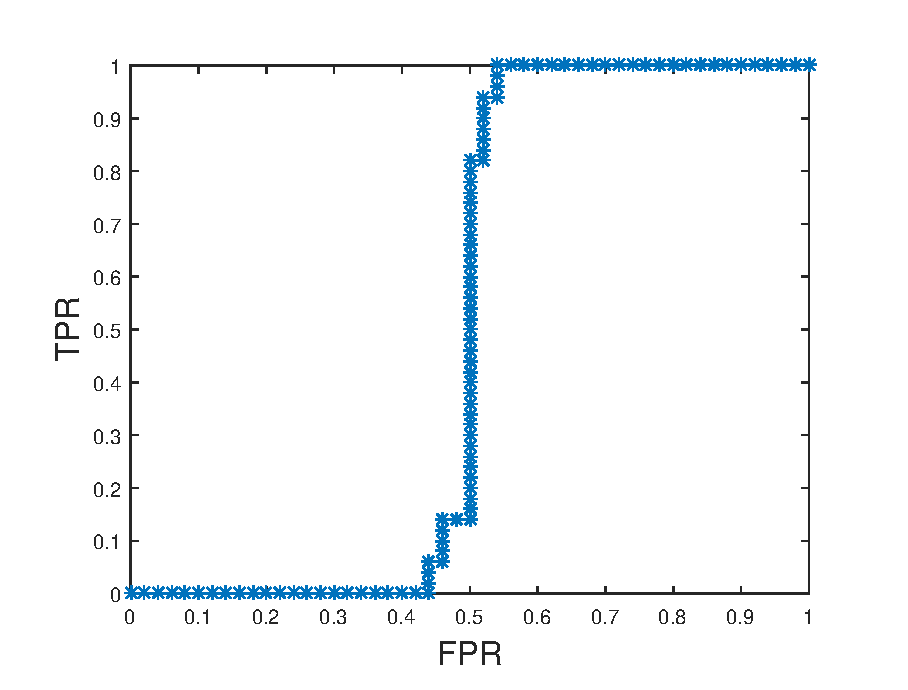
\includegraphics[width=0.6\textwidth]{figuras/prueba.eps}
	\caption{Pie de figura. Poner aquí cita del lugar de donde 
	se ha tomado la imagen en caso de que sea así. }
	\label{fig:prueba}
\end{figure}
\end{verbatim}

% Y ahora pongo la plantilla para que se incluya la figura efectivamente
\begin{figure}[t]
	\centering
	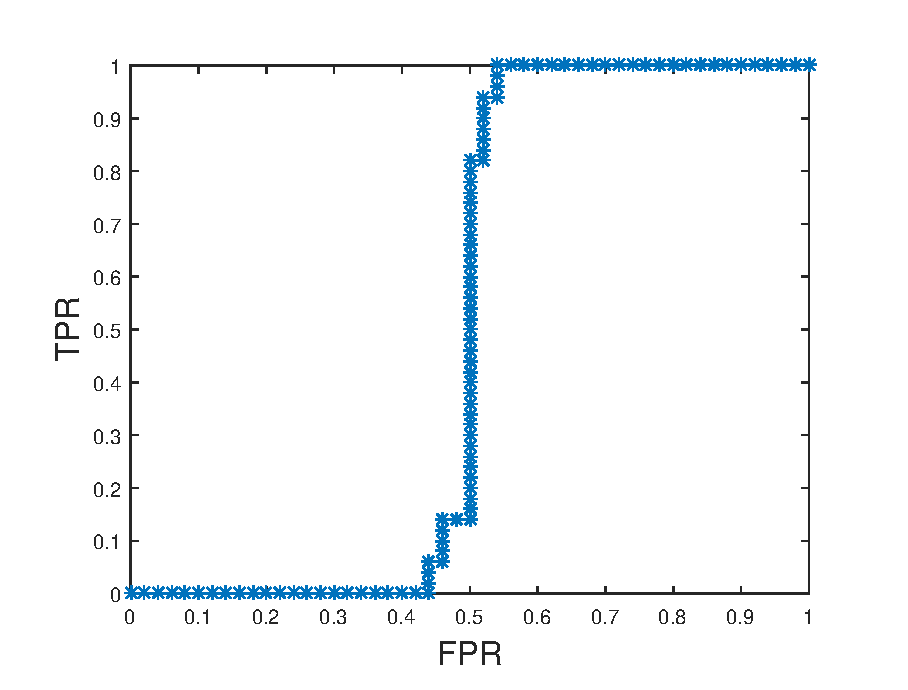
\includegraphics[width=0.6\textwidth]{figuras/prueba.eps}
	\caption{Pie de figura. Poner aquí cita del lugar de donde se ha tomado la imagen en caso de que sea así. }
	\label{fig:prueba}
\end{figure}

Si se pone el modificador [t] (top) latex ubicará la figura en la parte de arriba de la página. Ver otros modificadores como [h] (here) o [b] (bottom). Se pueden usar otras plantillas para, por ejemplo, poner dos figuras una al lado de otra. Consultar en Internet diferentes plantillas en caso de necesidad. 

Cuando en el texto nos refiramos a la figura en cuestión por el número, debemos usar la mayúscula y utilizar referencia a la figura. Esto hará que no nos tengamos que preocupar de la numeración de las figuras. Ej. Como se puede comprobar en la Figura~\ref{fig:prueba}.

Sustituir expresiones del tipo: “En la siguiente figura…” por “En la Figura 2.2…”


\subsection*{Inserción de tablas}

Este sería un ejemplo de una tabla. Se puede modificar el formato y contenido (ver en Internet algún enlace sobre cómo formatear tablas en latex). 

\begin{table}[t]
	\caption{Descripción de la tabla.}
	\label{table:prueba}
	\centering
	\begin{tabular}{l  c} 
		\hline \\[-1.5ex]
		\textbf{Tipo de ataque} & \textbf{Etiqueta} \\ [1ex] 
		\hline\hline \\[-1.5ex]
		DoS11 & dos \\ [0.5ex]
		Exf1MBp & exf1KB \\ [1ex]
		\hline
	\end{tabular}
\end{table}

La forma de referirse a las tablas es similar a las de las figuras (usar mayúsculas y referencia a la etiqueta(label) de la tabla). Ej. Como se puede ver en la Tabla~\ref{table:prueba}, ...


\subsection*{Citas de bibliografía}
Ejemplo de cita de bibliografía. Primero se va a google.scholar y se busca la referencia. Después se da al enlace citar, y se elige el formato bibtex. Se copia ese texto en el fichero bibliografia.bib. Un ejemplo de referenciar una cita es \cite{macia2008evaluation}.


\subsection*{Referencias a secciones}

Para referirnos a secciones, primero debemos tener una etiqueta de tipo \texttt{label} en dicha sección. Posteriormente, pondremos una referencia a dicho label, igual que hacemos para las figuras y las tablas. Ej. Como se ha mencionado en la Sección~\ref{sec:intro:motivacion} (Nótese que la palabra Sección va con mayúscula).

\subsection*{Glosario y acrónimos}

Cuando se utilice un acrónimo se debe definir en el fichero glosario/entradas\_glosario, tal y como está el ejemplo en dicho fichero. Al referirse en el texto se indicará así: \gls{svm} (ver que la primera vez lo pondrá completo). La segunda vez que se referencie a \gls{svm} ya no aparece completo. También se puede nombrar en plural así: \glspl{svm}. 
Otros ejemplos de acrónimo son: \gls{gcd}, \gls{lcm}, \gls{gmf}. 

A la hora de compilar con el glosario, se debe abrir una terminal CMD en el directorio de los fuentes latex del proyecto, y ejecutar el siguiente comando: \texttt{makeglossaries proyecto}. Esto generará los ficheros auxiliares que contienen el glosario. 

\subsection*{Listados de código}

Aquí se puede ver un ejemplo de listado de código: 

%\begin{lstlisting}[frame=none, numbers=none]


\begin{lstlisting}[language=Python,caption=Ejemplo de Python, label=listado:pythonPrueba]
import numpy as np

def incmatrix(genl1,genl2):
	m = len(genl1)
	n = len(genl2)
	M = None #to become the incidence matrix
	VT = np.zeros((n*m,1), int)  #dummy variable

	#compute the bitwise xor matrix
	M1 = bitxormatrix(genl1)
	M2 = np.triu(bitxormatrix(genl2),1) 
	
	for i in range(m-1):
		for j in range(i+1, m):
			[r,c] = np.where(M2 == M1[i,j])
			for k in range(len(r)):
				VT[(i)*n + r[k]] = 1;
				VT[(i)*n + c[k]] = 1;
				VT[(j)*n + r[k]] = 1;
				VT[(j)*n + c[k]] = 1;
	
	if M is None:
		M = np.copy(VT)
	else:
		M = np.concatenate((M, VT), 1)
	
	VT = np.zeros((n*m,1), int)
	
	return M

\end{lstlisting}

Nos podemos referir a él como Listado de código~\ref{listado:pythonPrueba}. 
Si queremos que aparezca como un flotante en la página debemos poner la palabra \texttt{float} así: 
\begin{verbatim}
\begin{lstlisting}[float,language=Python,caption=Ejemplo de Python, 
label=listado:pythonPrueba]
\end{verbatim}


\subsection*{Enlaces URL}
Podemos poner un enlace así \url{http://dtstc.ugr.es/~gmacia} --> %

\chapter*{Guía de estilo para escribir un TFG/TFM} \addcontentsline{toc}{chapter}{Guía de estilo}

Este capítulo no forma parte del TFG/TFM. Su único objetivo es aportar algunas recomendaciones y plantillas para tener claro cómo redactar el TFG/TFM. Una vez se haya comprendido, se puede comentar la siguiente línea en el fichero proyecto.tex añadiéndole al principio el carácter \%: 
\begin{verbatim}
\input{guiaDeEstilo} --> %\input{guiaDeEstilo}
\end{verbatim}

\section*{Recomendaciones generales}
A la hora de escribir el TFG/TFM es importante seguir las siguientes recomendaciones: 

\begin{enumerate}
	\item La memoria debe realizarse con el \textbf{máximo cuidado}, y debe proporcionar de forma consistente -y por sí misma- una idea clara y concisa de lo que se ha realizado. 
	\item No debe tener errores tipográficos ni ortográficos. Este es un aspecto que penaliza muchísimo el trabajo en la evaluación del tribunal. 
	\item Siempre que se utilice alguna figura no elaborada por el autor del proyecto debe indicarse la fuente de la que se ha sacado mediante una cita en la bibliografía. 
	\item La lectura debe ser fluida. Por ello, dada la dificultad que tiene afrontar la escritura de un texto largo casi por primera vez, se recomienda elaborar un índice rellenando los títulos de los diferentes apartados de que constará este documento. En segundo lugar, para cada apartado, se indicarán a modo de resumen las diferentes ideas que se desarrollarán posteriormente (una línea de texto por idea). Después, se desarrollan las ideas (cada idea en un párrafo). Cuando se termina, se realiza una lectura completa y detallada del texto para comprobar que es coherente y no tiene fallos ortográficos, tipográficos ni gramaticales, antes de pasarlo al tutor. 
	\item Una extensión normal está entorno a las 100-120 páginas. Esto no quiere decir que tengamos que escribir por escribir, ni meter contenido adicional sin sentido. Hay que escribir el proyecto de forma coherente, pero sin ser telegráfico, esto es, realizando una descripción detallada del trabajo realizado. 
	\item Evitar afirmaciones del tipo “El sistema diseñado es bastante bueno”. Esa misma frase debería ser escrita tal que responda a las preguntas: ¿Qué parte del sistema? ¿En qué sentido? ¿Cuánto de bueno? ¿Comparado con qué?
	\item Evitar la primera persona (incluso del plural). No obstante para resaltar la autoría de algo o enfatizar una posición personal sí se puede usar.
	\item Numerar estructuradamente los capítulos, secciones y subsecciones. Evitar más de tres niveles de anidamiento. 
	\item Toda afirmación categórica o se demuestra (teórica o experimentalmente)  o se incluye una referencia en la que se haya previamente demostrado.
	\item Toda tecnología, teorema, institución, norma, documento que se mencione debe estar referenciado. No incluir referencias a la wiki.
	\item Los términos en ingles que no tenga sentido traducir se pondrán en cursiva al menos para indicar que es un término no castellano.
	 

\end{enumerate}

\section*{Recomendaciones específicas para determinados contenidos}

\subsection*{Inserción de figuras}
Esta es una plantilla de código para adjuntar una figura. 

% El verbatim es solo para poner en el PDF el código que corresponde a la inserción de la figura
\begin{verbatim}
\begin{figure}[t]
	\centering
		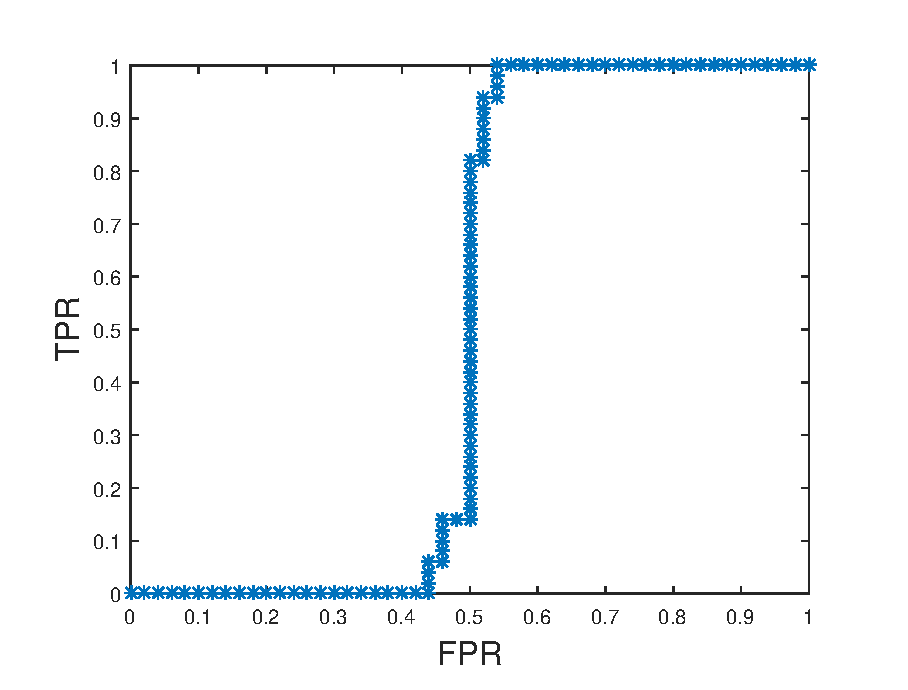
\includegraphics[width=0.6\textwidth]{figuras/prueba.eps}
	\caption{Pie de figura. Poner aquí cita del lugar de donde 
	se ha tomado la imagen en caso de que sea así. }
	\label{fig:prueba}
\end{figure}
\end{verbatim}

% Y ahora pongo la plantilla para que se incluya la figura efectivamente
\begin{figure}[t]
	\centering
	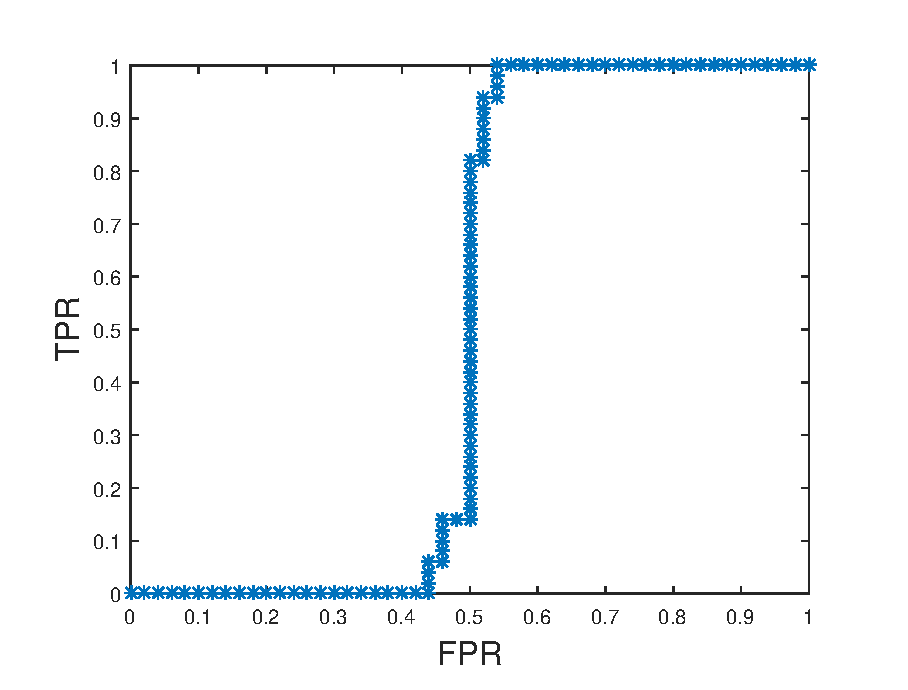
\includegraphics[width=0.6\textwidth]{figuras/prueba.eps}
	\caption{Pie de figura. Poner aquí cita del lugar de donde se ha tomado la imagen en caso de que sea así. }
	\label{fig:prueba}
\end{figure}

Si se pone el modificador [t] (top) latex ubicará la figura en la parte de arriba de la página. Ver otros modificadores como [h] (here) o [b] (bottom). Se pueden usar otras plantillas para, por ejemplo, poner dos figuras una al lado de otra. Consultar en Internet diferentes plantillas en caso de necesidad. 

Cuando en el texto nos refiramos a la figura en cuestión por el número, debemos usar la mayúscula y utilizar referencia a la figura. Esto hará que no nos tengamos que preocupar de la numeración de las figuras. Ej. Como se puede comprobar en la Figura~\ref{fig:prueba}.

Sustituir expresiones del tipo: “En la siguiente figura…” por “En la Figura 2.2…”


\subsection*{Inserción de tablas}

Este sería un ejemplo de una tabla. Se puede modificar el formato y contenido (ver en Internet algún enlace sobre cómo formatear tablas en latex). 

\begin{table}[t]
	\caption{Descripción de la tabla.}
	\label{table:prueba}
	\centering
	\begin{tabular}{l  c} 
		\hline \\[-1.5ex]
		\textbf{Tipo de ataque} & \textbf{Etiqueta} \\ [1ex] 
		\hline\hline \\[-1.5ex]
		DoS11 & dos \\ [0.5ex]
		Exf1MBp & exf1KB \\ [1ex]
		\hline
	\end{tabular}
\end{table}

La forma de referirse a las tablas es similar a las de las figuras (usar mayúsculas y referencia a la etiqueta(label) de la tabla). Ej. Como se puede ver en la Tabla~\ref{table:prueba}, ...


\subsection*{Citas de bibliografía}
Ejemplo de cita de bibliografía. Primero se va a google.scholar y se busca la referencia. Después se da al enlace citar, y se elige el formato bibtex. Se copia ese texto en el fichero bibliografia.bib. Un ejemplo de referenciar una cita es \cite{macia2008evaluation}.


\subsection*{Referencias a secciones}

Para referirnos a secciones, primero debemos tener una etiqueta de tipo \texttt{label} en dicha sección. Posteriormente, pondremos una referencia a dicho label, igual que hacemos para las figuras y las tablas. Ej. Como se ha mencionado en la Sección~\ref{sec:intro:motivacion} (Nótese que la palabra Sección va con mayúscula).

\subsection*{Glosario y acrónimos}

Cuando se utilice un acrónimo se debe definir en el fichero glosario/entradas\_glosario, tal y como está el ejemplo en dicho fichero. Al referirse en el texto se indicará así: \gls{svm} (ver que la primera vez lo pondrá completo). La segunda vez que se referencie a \gls{svm} ya no aparece completo. También se puede nombrar en plural así: \glspl{svm}. 
Otros ejemplos de acrónimo son: \gls{gcd}, \gls{lcm}, \gls{gmf}. 

A la hora de compilar con el glosario, se debe abrir una terminal CMD en el directorio de los fuentes latex del proyecto, y ejecutar el siguiente comando: \texttt{makeglossaries proyecto}. Esto generará los ficheros auxiliares que contienen el glosario. 

\subsection*{Listados de código}

Aquí se puede ver un ejemplo de listado de código: 

%\begin{lstlisting}[frame=none, numbers=none]


\begin{lstlisting}[language=Python,caption=Ejemplo de Python, label=listado:pythonPrueba]
import numpy as np

def incmatrix(genl1,genl2):
	m = len(genl1)
	n = len(genl2)
	M = None #to become the incidence matrix
	VT = np.zeros((n*m,1), int)  #dummy variable

	#compute the bitwise xor matrix
	M1 = bitxormatrix(genl1)
	M2 = np.triu(bitxormatrix(genl2),1) 
	
	for i in range(m-1):
		for j in range(i+1, m):
			[r,c] = np.where(M2 == M1[i,j])
			for k in range(len(r)):
				VT[(i)*n + r[k]] = 1;
				VT[(i)*n + c[k]] = 1;
				VT[(j)*n + r[k]] = 1;
				VT[(j)*n + c[k]] = 1;
	
	if M is None:
		M = np.copy(VT)
	else:
		M = np.concatenate((M, VT), 1)
	
	VT = np.zeros((n*m,1), int)
	
	return M

\end{lstlisting}

Nos podemos referir a él como Listado de código~\ref{listado:pythonPrueba}. 
Si queremos que aparezca como un flotante en la página debemos poner la palabra \texttt{float} así: 
\begin{verbatim}
\begin{lstlisting}[float,language=Python,caption=Ejemplo de Python, 
label=listado:pythonPrueba]
\end{verbatim}


\subsection*{Enlaces URL}
Podemos poner un enlace así \url{http://dtstc.ugr.es/~gmacia}
\end{verbatim}

\section*{Recomendaciones generales}
A la hora de escribir el TFG/TFM es importante seguir las siguientes recomendaciones: 

\begin{enumerate}
	\item La memoria debe realizarse con el \textbf{máximo cuidado}, y debe proporcionar de forma consistente -y por sí misma- una idea clara y concisa de lo que se ha realizado. 
	\item No debe tener errores tipográficos ni ortográficos. Este es un aspecto que penaliza muchísimo el trabajo en la evaluación del tribunal. 
	\item Siempre que se utilice alguna figura no elaborada por el autor del proyecto debe indicarse la fuente de la que se ha sacado mediante una cita en la bibliografía. 
	\item La lectura debe ser fluida. Por ello, dada la dificultad que tiene afrontar la escritura de un texto largo casi por primera vez, se recomienda elaborar un índice rellenando los títulos de los diferentes apartados de que constará este documento. En segundo lugar, para cada apartado, se indicarán a modo de resumen las diferentes ideas que se desarrollarán posteriormente (una línea de texto por idea). Después, se desarrollan las ideas (cada idea en un párrafo). Cuando se termina, se realiza una lectura completa y detallada del texto para comprobar que es coherente y no tiene fallos ortográficos, tipográficos ni gramaticales, antes de pasarlo al tutor. 
	\item Una extensión normal está entorno a las 100-120 páginas. Esto no quiere decir que tengamos que escribir por escribir, ni meter contenido adicional sin sentido. Hay que escribir el proyecto de forma coherente, pero sin ser telegráfico, esto es, realizando una descripción detallada del trabajo realizado. 
	\item Evitar afirmaciones del tipo “El sistema diseñado es bastante bueno”. Esa misma frase debería ser escrita tal que responda a las preguntas: ¿Qué parte del sistema? ¿En qué sentido? ¿Cuánto de bueno? ¿Comparado con qué?
	\item Evitar la primera persona (incluso del plural). No obstante para resaltar la autoría de algo o enfatizar una posición personal sí se puede usar.
	\item Numerar estructuradamente los capítulos, secciones y subsecciones. Evitar más de tres niveles de anidamiento. 
	\item Toda afirmación categórica o se demuestra (teórica o experimentalmente)  o se incluye una referencia en la que se haya previamente demostrado.
	\item Toda tecnología, teorema, institución, norma, documento que se mencione debe estar referenciado. No incluir referencias a la wiki.
	\item Los términos en ingles que no tenga sentido traducir se pondrán en cursiva al menos para indicar que es un término no castellano.
	 

\end{enumerate}

\section*{Recomendaciones específicas para determinados contenidos}

\subsection*{Inserción de figuras}
Esta es una plantilla de código para adjuntar una figura. 

% El verbatim es solo para poner en el PDF el código que corresponde a la inserción de la figura
\begin{verbatim}
\begin{figure}[t]
	\centering
		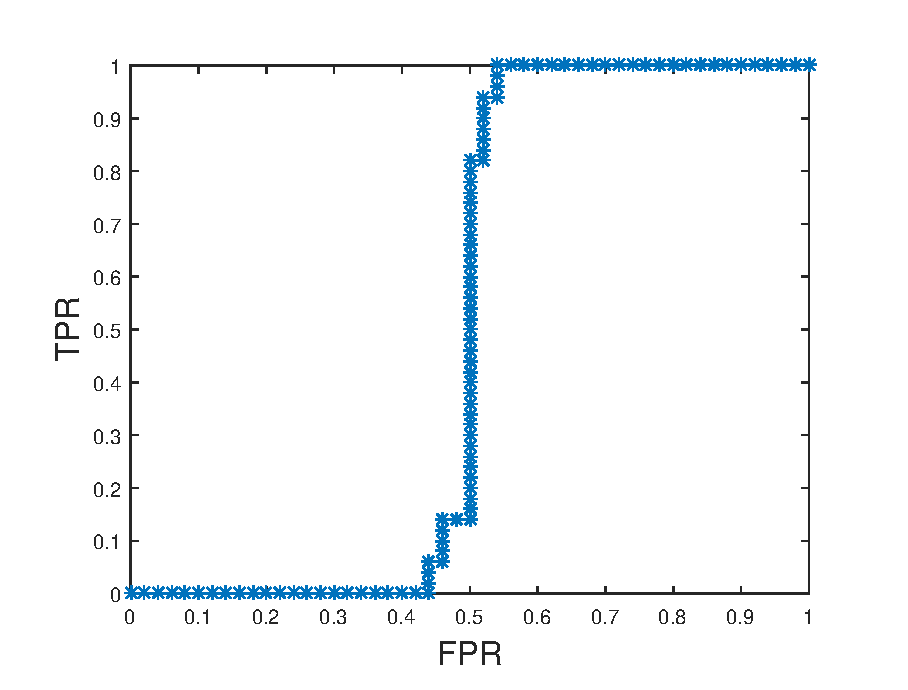
\includegraphics[width=0.6\textwidth]{figuras/prueba.eps}
	\caption{Pie de figura. Poner aquí cita del lugar de donde 
	se ha tomado la imagen en caso de que sea así. }
	\label{fig:prueba}
\end{figure}
\end{verbatim}

% Y ahora pongo la plantilla para que se incluya la figura efectivamente
\begin{figure}[t]
	\centering
	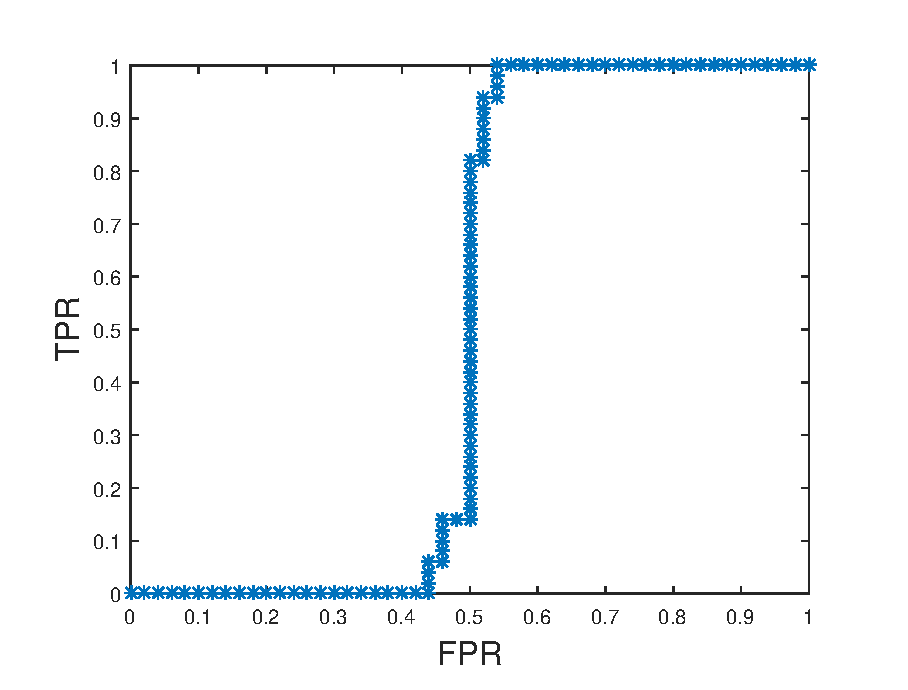
\includegraphics[width=0.6\textwidth]{figuras/prueba.eps}
	\caption{Pie de figura. Poner aquí cita del lugar de donde se ha tomado la imagen en caso de que sea así. }
	\label{fig:prueba}
\end{figure}

Si se pone el modificador [t] (top) latex ubicará la figura en la parte de arriba de la página. Ver otros modificadores como [h] (here) o [b] (bottom). Se pueden usar otras plantillas para, por ejemplo, poner dos figuras una al lado de otra. Consultar en Internet diferentes plantillas en caso de necesidad. 

Cuando en el texto nos refiramos a la figura en cuestión por el número, debemos usar la mayúscula y utilizar referencia a la figura. Esto hará que no nos tengamos que preocupar de la numeración de las figuras. Ej. Como se puede comprobar en la Figura~\ref{fig:prueba}.

Sustituir expresiones del tipo: “En la siguiente figura…” por “En la Figura 2.2…”


\subsection*{Inserción de tablas}

Este sería un ejemplo de una tabla. Se puede modificar el formato y contenido (ver en Internet algún enlace sobre cómo formatear tablas en latex). 

\begin{table}[t]
	\caption{Descripción de la tabla.}
	\label{table:prueba}
	\centering
	\begin{tabular}{l  c} 
		\hline \\[-1.5ex]
		\textbf{Tipo de ataque} & \textbf{Etiqueta} \\ [1ex] 
		\hline\hline \\[-1.5ex]
		DoS11 & dos \\ [0.5ex]
		Exf1MBp & exf1KB \\ [1ex]
		\hline
	\end{tabular}
\end{table}

La forma de referirse a las tablas es similar a las de las figuras (usar mayúsculas y referencia a la etiqueta(label) de la tabla). Ej. Como se puede ver en la Tabla~\ref{table:prueba}, ...


\subsection*{Citas de bibliografía}
Ejemplo de cita de bibliografía. Primero se va a google.scholar y se busca la referencia. Después se da al enlace citar, y se elige el formato bibtex. Se copia ese texto en el fichero bibliografia.bib. Un ejemplo de referenciar una cita es \cite{macia2008evaluation}.


\subsection*{Referencias a secciones}

Para referirnos a secciones, primero debemos tener una etiqueta de tipo \texttt{label} en dicha sección. Posteriormente, pondremos una referencia a dicho label, igual que hacemos para las figuras y las tablas. Ej. Como se ha mencionado en la Sección~\ref{sec:intro:motivacion} (Nótese que la palabra Sección va con mayúscula).

\subsection*{Glosario y acrónimos}

Cuando se utilice un acrónimo se debe definir en el fichero glosario/entradas\_glosario, tal y como está el ejemplo en dicho fichero. Al referirse en el texto se indicará así: \gls{svm} (ver que la primera vez lo pondrá completo). La segunda vez que se referencie a \gls{svm} ya no aparece completo. También se puede nombrar en plural así: \glspl{svm}. 
Otros ejemplos de acrónimo son: \gls{gcd}, \gls{lcm}, \gls{gmf}. 

A la hora de compilar con el glosario, se debe abrir una terminal CMD en el directorio de los fuentes latex del proyecto, y ejecutar el siguiente comando: \texttt{makeglossaries proyecto}. Esto generará los ficheros auxiliares que contienen el glosario. 

\subsection*{Listados de código}

Aquí se puede ver un ejemplo de listado de código: 

%\begin{lstlisting}[frame=none, numbers=none]


\begin{lstlisting}[language=Python,caption=Ejemplo de Python, label=listado:pythonPrueba]
import numpy as np

def incmatrix(genl1,genl2):
	m = len(genl1)
	n = len(genl2)
	M = None #to become the incidence matrix
	VT = np.zeros((n*m,1), int)  #dummy variable

	#compute the bitwise xor matrix
	M1 = bitxormatrix(genl1)
	M2 = np.triu(bitxormatrix(genl2),1) 
	
	for i in range(m-1):
		for j in range(i+1, m):
			[r,c] = np.where(M2 == M1[i,j])
			for k in range(len(r)):
				VT[(i)*n + r[k]] = 1;
				VT[(i)*n + c[k]] = 1;
				VT[(j)*n + r[k]] = 1;
				VT[(j)*n + c[k]] = 1;
	
	if M is None:
		M = np.copy(VT)
	else:
		M = np.concatenate((M, VT), 1)
	
	VT = np.zeros((n*m,1), int)
	
	return M

\end{lstlisting}

Nos podemos referir a él como Listado de código~\ref{listado:pythonPrueba}. 
Si queremos que aparezca como un flotante en la página debemos poner la palabra \texttt{float} así: 
\begin{verbatim}
\begin{lstlisting}[float,language=Python,caption=Ejemplo de Python, 
label=listado:pythonPrueba]
\end{verbatim}


\subsection*{Enlaces URL}
Podemos poner un enlace así \url{http://dtstc.ugr.es/~gmacia}
\end{verbatim}

\section*{Recomendaciones generales}
A la hora de escribir el TFG/TFM es importante seguir las siguientes recomendaciones: 

\begin{enumerate}
	\item La memoria debe realizarse con el \textbf{máximo cuidado}, y debe proporcionar de forma consistente -y por sí misma- una idea clara y concisa de lo que se ha realizado. 
	\item No debe tener errores tipográficos ni ortográficos. Este es un aspecto que penaliza muchísimo el trabajo en la evaluación del tribunal. 
	\item Siempre que se utilice alguna figura no elaborada por el autor del proyecto debe indicarse la fuente de la que se ha sacado mediante una cita en la bibliografía. 
	\item La lectura debe ser fluida. Por ello, dada la dificultad que tiene afrontar la escritura de un texto largo casi por primera vez, se recomienda elaborar un índice rellenando los títulos de los diferentes apartados de que constará este documento. En segundo lugar, para cada apartado, se indicarán a modo de resumen las diferentes ideas que se desarrollarán posteriormente (una línea de texto por idea). Después, se desarrollan las ideas (cada idea en un párrafo). Cuando se termina, se realiza una lectura completa y detallada del texto para comprobar que es coherente y no tiene fallos ortográficos, tipográficos ni gramaticales, antes de pasarlo al tutor. 
	\item Una extensión normal está entorno a las 100-120 páginas. Esto no quiere decir que tengamos que escribir por escribir, ni meter contenido adicional sin sentido. Hay que escribir el proyecto de forma coherente, pero sin ser telegráfico, esto es, realizando una descripción detallada del trabajo realizado. 
	\item Evitar afirmaciones del tipo “El sistema diseñado es bastante bueno”. Esa misma frase debería ser escrita tal que responda a las preguntas: ¿Qué parte del sistema? ¿En qué sentido? ¿Cuánto de bueno? ¿Comparado con qué?
	\item Evitar la primera persona (incluso del plural). No obstante para resaltar la autoría de algo o enfatizar una posición personal sí se puede usar.
	\item Numerar estructuradamente los capítulos, secciones y subsecciones. Evitar más de tres niveles de anidamiento. 
	\item Toda afirmación categórica o se demuestra (teórica o experimentalmente)  o se incluye una referencia en la que se haya previamente demostrado.
	\item Toda tecnología, teorema, institución, norma, documento que se mencione debe estar referenciado. No incluir referencias a la wiki.
	\item Los términos en ingles que no tenga sentido traducir se pondrán en cursiva al menos para indicar que es un término no castellano.
	 

\end{enumerate}

\section*{Recomendaciones específicas para determinados contenidos}

\subsection*{Inserción de figuras}
Esta es una plantilla de código para adjuntar una figura. 

% El verbatim es solo para poner en el PDF el código que corresponde a la inserción de la figura
\begin{verbatim}
\begin{figure}[t]
	\centering
		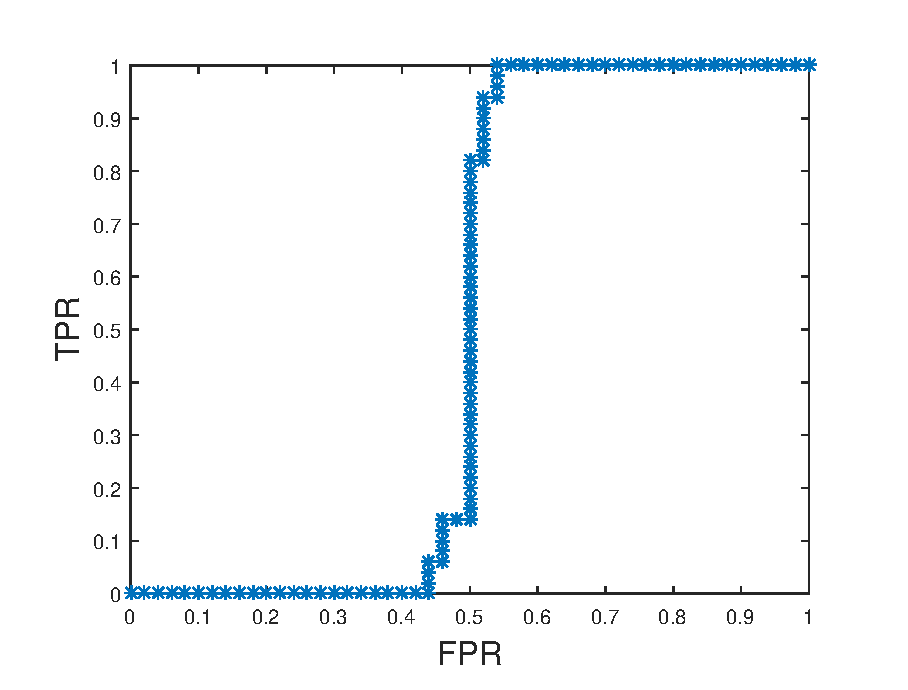
\includegraphics[width=0.6\textwidth]{figuras/prueba.eps}
	\caption{Pie de figura. Poner aquí cita del lugar de donde 
	se ha tomado la imagen en caso de que sea así. }
	\label{fig:prueba}
\end{figure}
\end{verbatim}

% Y ahora pongo la plantilla para que se incluya la figura efectivamente
\begin{figure}[t]
	\centering
	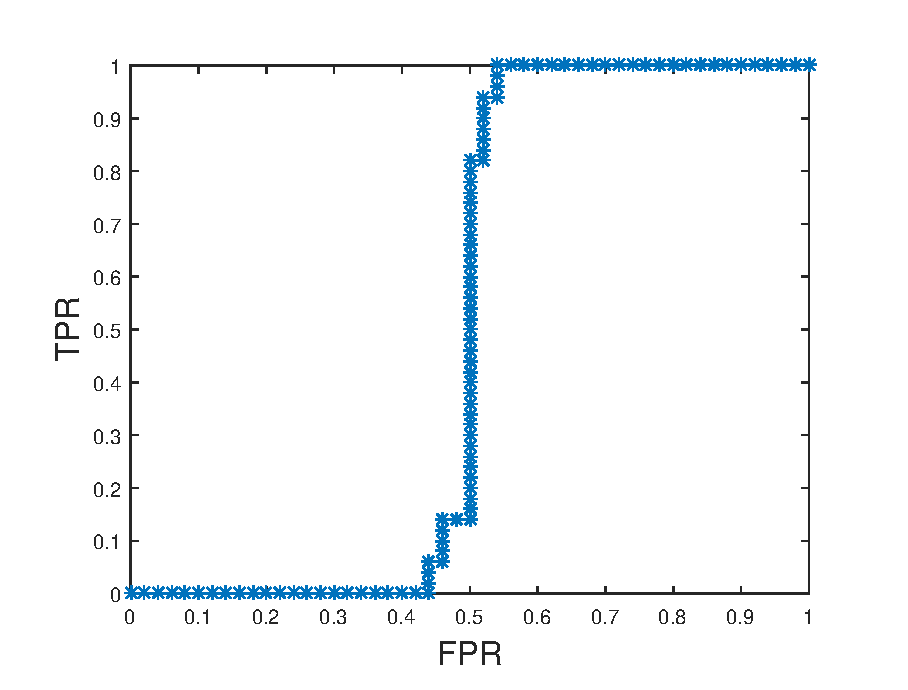
\includegraphics[width=0.6\textwidth]{figuras/prueba.eps}
	\caption{Pie de figura. Poner aquí cita del lugar de donde se ha tomado la imagen en caso de que sea así. }
	\label{fig:prueba}
\end{figure}

Si se pone el modificador [t] (top) latex ubicará la figura en la parte de arriba de la página. Ver otros modificadores como [h] (here) o [b] (bottom). Se pueden usar otras plantillas para, por ejemplo, poner dos figuras una al lado de otra. Consultar en Internet diferentes plantillas en caso de necesidad. 

Cuando en el texto nos refiramos a la figura en cuestión por el número, debemos usar la mayúscula y utilizar referencia a la figura. Esto hará que no nos tengamos que preocupar de la numeración de las figuras. Ej. Como se puede comprobar en la Figura~\ref{fig:prueba}.

Sustituir expresiones del tipo: “En la siguiente figura…” por “En la Figura 2.2…”


\subsection*{Inserción de tablas}

Este sería un ejemplo de una tabla. Se puede modificar el formato y contenido (ver en Internet algún enlace sobre cómo formatear tablas en latex). 

\begin{table}[t]
	\caption{Descripción de la tabla.}
	\label{table:prueba}
	\centering
	\begin{tabular}{l  c} 
		\hline \\[-1.5ex]
		\textbf{Tipo de ataque} & \textbf{Etiqueta} \\ [1ex] 
		\hline\hline \\[-1.5ex]
		DoS11 & dos \\ [0.5ex]
		Exf1MBp & exf1KB \\ [1ex]
		\hline
	\end{tabular}
\end{table}

La forma de referirse a las tablas es similar a las de las figuras (usar mayúsculas y referencia a la etiqueta(label) de la tabla). Ej. Como se puede ver en la Tabla~\ref{table:prueba}, ...


\subsection*{Citas de bibliografía}
Ejemplo de cita de bibliografía. Primero se va a google.scholar y se busca la referencia. Después se da al enlace citar, y se elige el formato bibtex. Se copia ese texto en el fichero bibliografia.bib. Un ejemplo de referenciar una cita es \cite{macia2008evaluation}.


\subsection*{Referencias a secciones}

Para referirnos a secciones, primero debemos tener una etiqueta de tipo \texttt{label} en dicha sección. Posteriormente, pondremos una referencia a dicho label, igual que hacemos para las figuras y las tablas. Ej. Como se ha mencionado en la Sección~\ref{sec:intro:motivacion} (Nótese que la palabra Sección va con mayúscula).

\subsection*{Glosario y acrónimos}

Cuando se utilice un acrónimo se debe definir en el fichero glosario/entradas\_glosario, tal y como está el ejemplo en dicho fichero. Al referirse en el texto se indicará así: \gls{svm} (ver que la primera vez lo pondrá completo). La segunda vez que se referencie a \gls{svm} ya no aparece completo. También se puede nombrar en plural así: \glspl{svm}. 
Otros ejemplos de acrónimo son: \gls{gcd}, \gls{lcm}, \gls{gmf}. 

A la hora de compilar con el glosario, se debe abrir una terminal CMD en el directorio de los fuentes latex del proyecto, y ejecutar el siguiente comando: \texttt{makeglossaries proyecto}. Esto generará los ficheros auxiliares que contienen el glosario. 

\subsection*{Listados de código}

Aquí se puede ver un ejemplo de listado de código: 

%\begin{lstlisting}[frame=none, numbers=none]


\begin{lstlisting}[language=Python,caption=Ejemplo de Python, label=listado:pythonPrueba]
import numpy as np

def incmatrix(genl1,genl2):
	m = len(genl1)
	n = len(genl2)
	M = None #to become the incidence matrix
	VT = np.zeros((n*m,1), int)  #dummy variable

	#compute the bitwise xor matrix
	M1 = bitxormatrix(genl1)
	M2 = np.triu(bitxormatrix(genl2),1) 
	
	for i in range(m-1):
		for j in range(i+1, m):
			[r,c] = np.where(M2 == M1[i,j])
			for k in range(len(r)):
				VT[(i)*n + r[k]] = 1;
				VT[(i)*n + c[k]] = 1;
				VT[(j)*n + r[k]] = 1;
				VT[(j)*n + c[k]] = 1;
	
	if M is None:
		M = np.copy(VT)
	else:
		M = np.concatenate((M, VT), 1)
	
	VT = np.zeros((n*m,1), int)
	
	return M

\end{lstlisting}

Nos podemos referir a él como Listado de código~\ref{listado:pythonPrueba}. 
Si queremos que aparezca como un flotante en la página debemos poner la palabra \texttt{float} así: 
\begin{verbatim}
\begin{lstlisting}[float,language=Python,caption=Ejemplo de Python, 
label=listado:pythonPrueba]
\end{verbatim}


\subsection*{Enlaces URL}
Podemos poner un enlace así \url{http://dtstc.ugr.es/~gmacia}
	\chapter{Introducción}


\section{Motivación y contexto del proyecto}
\label{sec:intro:motivacion} %Esto se pone si queremos hacer referencia a esta sección

En esta parte es importante clarificar las siguientes preguntas: 
\begin{enumerate}
\item ¿Cuál es el problema que pretendemos resolver con este proyecto? Debemos introducir un poco el contexto en el que aparece y describir bien en qué consiste dicho problema. 
\item ¿Por qué es importante dicho problema? Hay que tratar de aportar datos y argumentos para indicar que el problema descrito es relevante en el contexto actual. 
\end{enumerate}

Este trabajo surge de la necesidad de disminuir las vulnerabilidades de los algoritmos criptográficos a ataques cuánticos. Así pues, el objetivo de este trabajo es modificar la implementación de la \textit{Blockchain} ARK para hacerla resistente a ataques cuanticos, con ayuda del sistema criptográfico PICNIC.

El desarrollo del trabajo se basa en dos tecnologías la computación cuántica y las cadenas de bloques. En primer lugar vamos a tratar la computación cuántica, se basa en el uso de cubits y hace posible que existan nuevos algoritmos que puedan resolver problemas con una complejidad mayor.

El origen de la computación cuántica surge de la necesidad de descubrir nuevas tecnologías, debido a que la evolución de la tecnología en los últimos años se ha basado en la reducción del tamaño de los transistores, aumentando así la velocidad del proyecto. El problema es que este proceso tiene un tiene un límite.

El estudio de las tecnologías cuánticas se inició en 1980, al principio se imaginaban ordenadores tradicionales que trabajaran con algunos principios de la mecánica cuántica.

En 1998 se consiguió analiza la información que transportaban los cúbits y ejecutar el algoritmo de búsqueda de Grover.

En 2019 IBM presenta el primer ordenador cuántico para uso comercial, que combina tanto la computación cuántica como tradicional para su utilización en invastigaciones y grandes cálculos.



Así mismo la otra tecnología que vamos a utilizar son las cadenas de bloques. Surgieron en la segunda década del siglo XXI, ha sido motor de cambio en el ámbito digital 





\section{Objetivos del proyecto y logros conseguidos}

Debemos poner claramente el objetivo del proyecto, sin muchos rodeos, para que esté claro desde el principio. A veces podemos tener un objetivo general (amplio) y algunos objetivos específicos (más concretos). 

Adicionalmente, debemos aportar información a los evaluadores y lectores de la memoria de cuál es el trabajo que hemos realizado nosotros en este proyecto. Por ello, se debe poner una lista de los ``logros conseguidos''. Un ejemplo: 

\begin{itemize}
	\item Se ha diseñado un sistema que permite...
	\item Se ha modificado un software existente para conseguir...
	\item Se ha desarrollado una interfaz gráfica para el acceso...
\end{itemize}


El objetivo principal es profundizar en estudio de las cadenas de bloques. Además se estudiará el algoritmo para usarlo en la impletación de la Blockchain y hacerla más segura.


\section{Estructura de la memoria}
Se describirán los capítulos que tiene la memoria, indicando qué contenidos habrá en cada uno de ellos, para permitir al lector situarse ante el documento. 


\section{Contenidos teóricos para la comprensión del proyecto}
En esta sección se realizará el desarrollo de los contenidos teóricos que permitan al lector entender el desarrollo del proyecto. Es importante no enrollarse con cosas que no tienen nada que ver con el proyecto. También es importante no copiar texto de otras fuentes si no están citadas.


Conceptos clave:

Contratos inteligentes: Base de "propiedades inteligentes" que permiten definir mediante códigos de la Blockchain, la forma en la que los dispositivos reaccionan ante eventos que tienen lugar en su entorno. Llevan incorporada una máquina virtual que habilita la codificación y ejecución de programas software para determinar las condiciones sobre el intercambio de activos entre agentes.

Firma electrónica: Sirve para controlar la integridad de los datos y asegurar que la información procede de quien dice ser su remitente, garantiza que la información que se almacena o se envía no ha sido modificada. Controla la auditoría del documento. Se requieren criptosistemas aritméticos

Criptosistemas aritméticos: Cada usuario posee una clave pública y otra privada. El usuario cifrará y descifrará el mensaje con su llave privada y pública, además de la llave pública del usuario que descifrará o que haya cifrado el mensaje.


Resumen o Hash: Es el resultado de aplicar una función que transforma un mensaje que longitud variable en uno de longitud fija, denominada función hash. Es el resultado de calcular el resto módulo n con n la longitud fija. Al aplicar la función hash a un fichero, si se modifica algún dato del mismo cambiará su hash y por tanto se sabrá si ha sido manipulado desde que se envió. Así podemos conseguir la integridad del mensaje

Blockchain: Sistemas de almacenamiento de información que se divide en bloque de datos enlazados mediante los hash. A cada bloque se le asocia un hash y contiene el hash del bloque anterior, creando una lista enlazada, la búsqueda de información no es muy óptima si hay un número elevado de bloques. Para ello existen los árboles merkle.
Los blockchain por si mismo no solucionan los problemas de los sistemas de la información y la comunicación. Pero permiten impulsar modificaciones orientadas a crear soluciones más robustas, implicando conocer donde hay que usar las blockchain y cual es la infraestructura.


Árboles Merkle: Árboles binarios con funciones hash, cada nodo tiene con máximo dos hijos, no hay ciclos. El cálculo de los hash de los padres se hace combinando los hash de los hijos. La integridad se obtiene inclueyendo en los bloques el valor del nodo raiz en lugar de añadir el valor de todos los datos protegidos por los bloques, reducimos además la información de la cabecera.




Bibliografia:

https://es.wikipedia.org/wiki/Computaci%C3%B3n_cu%C3%A1ntica

	\chapter{Planificación y costes}

Definir claramente de acuerdo con el tutor los “paquetes de trabajo” (PTs), identificando claramente los entregables resultantes de cada uno de ellos. Esto definirá claramente los resultados del proyecto. Pueden usarse Diagramas de Gantt o cualquier herramienta o metodología siempre que facilite la visualización secuencial y dependencias entre los PT. En este mismo capítulo se incluir un presupuesto –ajustado en lo posible a la realidad- que incluya recursos humanos y materiales, así como cualquier dato que determine la viabilidad del proyecto.

	\chapter{Análisis del problema}


\section{Especificación de requisitos}

Debe incluir una clara descripción de las funcionalidades que se esperan alcanzar, así como las restricciones o condicionantes que puedan determinar el diseño o solución adoptada. Tras eso deben especificarse claramente los requisitos.

Los requisitos pueden ser funcionales (e.g. La herramienta debe mostrar las medidas de la red en tiempo real), o no funcionales (e.g. se debe garantizar el acceso seguro a la herramienta; el rendimiento debe ser alto; el consumo de memoria debe ser bajo; etc.)



\subsection{Requisitos funcionales}

\begin{table}[H]
	\begin{center}
	\centering
	\resizebox{\linewidth}{!}{
	\begin{tabular}{p{0.14\linewidth} p{0.75\linewidth}}
		\textbf{Requisito} & \textbf{Descripción} \\
		\toprule
		RF 1.1 & El programa deberá de generar la clave pública y privada de cada usuario\\[0.5ex]
		RF 1.2 & El programa deberá de firmar correctamente cada \textit{hash}, ya sea de un mensaje o una transacción\\[0.5ex]
		RF 1.3 & El programa deberá de realizar correctamente la verificación del \textit{hash}\\[0.5ex]
		\bottomrule
	\end{tabular}}
	\end{center}
	\caption{Requisitos del programa}
\end{table}


\begin{table}[H]
	\begin{center}
	\centering
	\resizebox{\linewidth}{!}{
	\begin{tabular}{p{0.14\linewidth} p{0.75\linewidth}}
		\textbf{Requisito} & \textbf{Descripción} \\
		\toprule
		RF 2.1 & La base de datos local del docker deberá almacenar la claves del usuario\\[0.5ex]
		RF 2.2 & La base de datos local del docker deberá almacenar la información del usuario\\[0.5ex]
		RF 2.2 & La base de datos local del docker deberá almacenar los monederos así como el saldo de cada usuario\\[0.5ex]
		RF 2.3 & El docker deberá de almacenar la \textit{blockchain}\\[0.5ex]
		RF 2.4 & El docker deberá mantener activa la ejecución de la \textit{blockchain}\\[0.5ex]
		RF 2.5 & El docker deberá mantener activa la ejecución del \textit{explorer}\\[0.5ex]
		RF 2.6 & El docker deberá mantener activos los puertos del explorer y API\\[0.5ex]
		\bottomrule
	\end{tabular}}
	\end{center}
	\caption{Requisitos del docker}
\end{table}

\begin{table}[H]
	\begin{center}
	\centering
	\resizebox{\linewidth}{!}{
	\begin{tabular}{p{0.14\linewidth} p{0.75\linewidth}}
		\textbf{Requisito} & \textbf{Descripción} \\
		\toprule
		RF 3.1 & La aplicación deberá dar la opción al usuario de crear un perfil\\[0.5ex]
		RF 3.2 & La aplicación deberá dar la opción al usuario de conectarse a la red \textit{testnet}\\[0.5ex]
		RF 3.3 & La aplicación deberá dar la opción al usuario de crear monederos\\[0.5ex]
		RF 3.4 & La aplicación deberá dar la opción al usuario realizar transacciones entre diferentes monederos\\[0.5ex]
		RF 3.5 & La aplicación deberá dar la opción al usuario de firmar mensajes\\[0.5ex]
		RF 3.6 & La aplicación deberá dar la opción al usuario de validar mensajes\\[0.5ex]
		\bottomrule
	\end{tabular}}
	\end{center}
	\caption{Requisitos de la aplicación Wallet}
\end{table}


\subsection{Requisitos no funcionales}

\begin{table}[H]
	\begin{center}
	\centering
	\resizebox{\linewidth}{!}{
	\begin{tabular}{p{0.14\linewidth} p{0.7\linewidth}}
		\textbf{Requisito} & \textbf{Descripción} \\
		\toprule
		RNF 1.1 & El programa no deberá de tardar más de medio minuto par de segundos en generar las claves públicas y privadas \\[0.5ex]
		RNF 1.2 & El programa deberá de tardar unos segundos en firmar un mensaje\\[0.5ex]
		RNF 1.3 & El programa deberá de tardar unos segundos en verificar la firma de un $hash$\\[0.5ex]
		RNF 1.4 & El programa deberá de ser correctamente integrado en el sistema \textit{blockchain}\\[0.5ex]
		
		RNF 1.5 & El programa deberá de ser compatible con cualquier sistema compatible con \texttt{python}\\[0.5ex]
		RNF 1.6 & La aplicación deberá de realizar transacciones de forma segura\\[0.5ex]
		RNF 1.7 & El proyecto deberá de contar con un manual de usuario claro y conciso\\[0.5ex]
		\bottomrule
	\end{tabular}}
	\end{center}
	\caption{Requisitos no funcionales}
\end{table}

\section{Análisis}

El objetivo de este apartado es mostrar en diferentes subapartados los diferentes subproblemas que han aparecido al realizar el proyecto, describiendo las alternativas que se han considerado, y justificando las decisiones que se han adoptado. A veces, especialmente cuando los conceptos utilizados en este apartado son extensos, es necesario clarificarlos previamente en el Capítulo de \textit{Introducción} (sección \textit{Contenidos teóricos para la comprensión del proyecto}).   
	\chapter{Diseño}

Es uno de los capítulos más importantes. Debe explicar claramente la solución propuesta justificando la aproximación adoptada. Este capítulo, según el caso, es aconsejable que defina claramente la arquitectura del sistema propuesto, identificando los roles o partes o actores del sistema. Pueden emplearse metodologías basadas en diagramas de clases, paquetes, diagramas secuenciales, diagramas de relación, etc.

Si se ha diseñado una interfaz gráfica debe también describirse su estructura, dónde se mostrará la información, etc.


	\chapter{Implementación}
\label{sec:implementacion}
%Aquí se deben proporcionar los detalles de cómo se ha llevado a la práctica el diseño propuesto en el capítulo anterior. Deben identificarse claramente herramientas, tecnologías, equipamientos, etc. utilizados o necesarios para el buen funcionamiento de la solución. Se pueden describir los fragmentos de código más importantes, con el fin de clarificar la funcionalidad que proporcionan. En general este capítulo debe facilitar la reutilización de nuestra solución, por lo que debe estar bien documentada. Puede incluir un manual de uso.


\section{Cuerpos finitos} % revisar con javier
Se trabajará con el cuerpo finito de 128 elementos, $\GF(2^7)$, que es un cuerpo extendido de $\GF(2)$ que corresponde con el cociente 
\begin{equation}
\GF(128) = \frac{\GF(2)[x]}{\langle x^7 + x + 1 \rangle}
\end{equation}

Además el orden del cuerpo de las unidades es $127$, que es primo entonces todo elemento del cuerpo distinto de $1$ es un elemento primitivo, es decir, un generador.

La tabla \ref{tab:rel} muestra una representación de los elementos no nulos del cuerpo. En la implementación se ha utilizado la representación como cadena de bits, puesto que a la hora de trabajar es más fácil con una cadeba de bits que con los polinomios.

\begin{table}[h]
\caption{Representación de los elementos no nulos del cuerpo finito de $2^7$ elementos}
\label{tab:rel}
\begin{center}
\begin{tabular}{p{0.16\linewidth}p {0.2\linewidth}p{0.2\linewidth}}
	 \textbf{Polinomio} & \textbf{Bits} & \textbf{$\log_a$}\\
\toprule
	$1$ & [0, 0, 0, 0, 0, 0, 1] & 0\\
	$a$ & [0, 0, 0, 0, 0, 1, 0] & 1\\
	$a^2$ & [0, 0, 0, 0, 1, 0, 0] & 2\\
	\\
	$\vdots$ & $\vdots$ & $\vdots$\\
	\\
	$a^6 + a^5 + a^4 + 1$ & [1, 1, 1, 0, 0, 0, 1] & 124\\
	$a^6 + a^5 + 1$ & [1, 1, 0, 0, 0, 0, 1] & 125\\
	$a^6 + 1$ & [1, 0, 0, 0, 0, 0, 1] & 126\\
\bottomrule
\end{tabular}
\end{center}


\end{table}

La implementación del cuerpo finito de $2^7$ elementos no se ha realizado de forma genérica sino para que sea específica para el algoritmo UOV, de esta forma es mucho más sencillo implementar la aritmética del cuerpo. Para la suma en $\mathds{Z}_2$ sólo tenemos que fijarnos que es lo mismo que el operador lógico \textit{XOR}, mientras que para el producto, al encontrarmos en un cuerpo como un orden pequeño, se usarán unas tablas que contienen las correspondencias entre los elementos no nulos del cuerpo y sus logaritmos en base $a$, por lo que el producto se convierte en una suma módulo $127$.




\section{Parámetros y fórmula}
Para empezar indicamos los parámetros que serán de utilidad para entender el algoritmo.
\begin{itemize}
	\item r: Grado del cuerpo extendido, $\mathds{F}_2 \subset \mathds{F}_{2^r}$. % quitar el F_2
	\item $x$: Vector de $n$ componentes, denominando a las primeras $v$ componentes  $x_1, \dotsb, x_v$ vinagre y al resto aceites.
	
	\item m: Tamaño de la clave pública, además del número de variables de aceite.
	\item $v$: Número de variables vinagre.
	%\item $\mathcal{H}$: Función salida extensible se usa para crear el hash del mensaje y proviene de la clave pública.
	%\item $\mathcal{G}$: Función salida extensible se usa para la generación de la clave pública a partir de una semilla pública.
\end{itemize}

$\mathcal{P}: \mathds{F}_{2^r}^n \rightarrow \mathds{F}_{2^r}^m$, esta función se puede descomponer como $\mathcal{P} = \mathcal{F} \circ \mathcal{T}$, donde $\mathcal{T}: \mathds{F}_{2^r}^n \rightarrow \mathds{F}_{2^r}^n$ es invertible, y $\mathcal{F}: \mathds{F}_{2^r}^n \rightarrow \mathds{F}_{2^r}^m$ siendo sus $m$ componentes de la forma:

\begin{equation}\label{eq:fun}
f_k(x) = \sum_{i=1}^v \sum_{j=i}^n \alpha_{i,j,k} x_i x_j + \sum_{i=1}^n \beta_{i,k} x_i
\end{equation}

donde $\alpha_{i,j,k}$ y $\beta_{i,k}$ se toman aleatoriamente en $\mathds{F}_2$ siendo $\alpha$ una matriz triangular superior. De esta manera será más eficiente y no afectará a la seguridad del algoritmo.



\section{Generación de la clave privada}
La clave privada está formada por $\alpha_{i,j,k}$ y $\beta_{i,k}$ que son valores del cuerpo $\mathds{F}_2$, tomados de forma aleatoria.


\section{Generación de la clave pública}
Generaremos una clave pública partiendo de la clave privada $\alpha_{i,j,k}$ y $\beta_{i,k}$.

Para entenderlo mejor ponemos las $m$ ecuaciones (\ref{eq:fun}) en forma matricial,

\begin{equation}\label{eq:matriz} 
f_k(x) = x^v\ [\alpha_{i,j,k}]\ (x^v, x^m)' + [\beta_{i,k}]\ (x^v, x^m)'
\end{equation}

siendo $[\alpha_{i,j,k}]$ y $[\beta_{i,k}]$ son las representaciones matriciales de $\alpha_{i,j,k}$ y $\beta_{i,k}$, $x^v$ los vinagres y $x^m$ los aceites, así $x$ se puede expresar como $(x^v, x^m)'$.

Conociendo los valores de la clave privada $\alpha$ y $\beta$, tomando de forma aleatoria los del vinagre $x^v$, los cuales pasaremos a denominarlos como $a^v$, y tomando los $m$ primeros bits del hash del mensaje $h_k$ podemos generar la clave pública.

Hacemos el cambio de notación $A_k = a^v\ [\alpha_{i,j,k}] = (A^v_k, A^m_k)$,  lo sustituimos en la ecuación (\ref{eq:matriz}) y despejamos los aceites.

\begin{align}
h_k &= A_k^v\ (a^v)' +  A_k^m\ (x^m)' + \beta_k^v\ (a^v)' + \beta_k^m\ (x^m)' + \gamma_k\\
(A_k^m + \beta_k^m) (x^m)' &= h_k - (A_k^v + \beta_k^v) (a^v)' -\gamma_k\\
\label{eq:despeje}
(x^m)' &= (A_k^m + \beta_k^m)^{-1} (h_k - (A_k^v + \beta_k^v) (a^v)' -\gamma_k)
\end{align}

Si $(A_k^m + \beta_k^m)$ fuese una matriz singular, entonces se tomarían otros valores de vinagres.


Para generar la clave pública necesitamos incluir una nueva matriz $T$, donde $T \cdot s' = x'$. Incluimos esta matriz $T$ para aumentar la seguridad del algoritmo y así sea más complejo calcular la función inversa $\mathcal{P}$

\begin{equation}
	T =
	\left[
	\begin{array}{c|c}
	I_v & T_{vxm} \\
	\hline
	0 & I_m
	\end{array}
	\right]
	\label{mat:T}
\end{equation}

Despejando x, obtenemos:

\begin{equation}
	x =  s \cdot T' = s  \left[
	\begin{array}{c|c}
	I_v & 0 \\
	\hline
	T'_{v x m} & I_m
	\end{array}
	\right]
	= [s^v, s^m] \left[
	\begin{array}{c|c}
	I_v & 0 \\
	\hline
	T'_{v x m} & I_m
	\end{array}
	\right]
	= (s^v + s^m T'_{vxm}, s^m )
\end{equation}

Sustituimos en (\ref{eq:matriz}):

\begin{equation}
	f_k(x) = s  \left[
	\begin{array}{c}
	I_v \\
	\hline
	T'_{v x m}
	\end{array}
	\right] [\alpha_{i,j,k}]_{\begin{subarray}{l}{1<i<v }\\ {i<j<n}\end{subarray}}\ T \ s' + [\beta_{j,k}]_{1<j<n}\ T\ s'
\end{equation}
donde $k \in \{1,...,m\}$

Así obtenemos las claves públicas definidas para cada $k$

\begin{itemize}
	\item ${\alpha_{pub}}_k = \left[
	\begin{array}{c}
	I_v \\
	\hline
	T'_{v x m}
	\end{array}
	\right] [\alpha_{i,j,k}]_{\begin{subarray}{l}{1<i<v }\\ {i<j<n}\end{subarray}} \ T$
	
	\item ${\beta_{pub}}_k = [\beta_{j,k}]_{1<j<n}\ T$

\end{itemize}


\section{Algoritmo de firma}
Por la definición de $x$ obtenemos la firma $s$ como

\begin{equation}
	s = x \cdot T'^{-1}
\end{equation}

donde $x = (x^v, x^m)$ con $x^v$ son los vinagres aleatorios y $x^m$ los aceites que hemos calculado en la ecuación (\ref{eq:despeje}).




\section{Algoritmo de verificación}

Para comprobar que el mensaje es correcto y que no ha sufrido ninguna transformación durante el envío del mismo, se tiene que cumplir la igualdad (\ref{eq:veri}).


\begin{equation}\label{eq:veri}
	h_k = \ {\alpha_{pub}}_k \ s' + {\beta_{pub}}_{k} \ s'
\end{equation}



	\chapter{Evaluación y pruebas}

En este capítulo se debe proporcionar una medida objetiva de las bondades y beneficios de la solución propuesta, tanto en términos absolutos, como –en la medida de lo posible- comparándola con otras soluciones. Dependiendo del tipo de proyecto, debe incluir los resultados experimentales obtenidos al probar la solución; también puede incluir una tabla o diagrama de los costes reales del desarrollo, para así establecer conclusiones respecto a la planificación y costes estimados a priori. Finalmente, cuando se trata del desarrollo de una aplicación software, se pueden definir baterías de pruebas a realizar, de modo que en este capítulo se especificarán qué pruebas se han realizado, los resultados esperados y los resultados obtenidos. 

	
\chapter{Conclusiones}

Capítulo en el que deben resumirse las principales aportaciones del trabajo realizado.


\section{Valoración personal}
Se puede incluir una valoración personal del proyecto (opcionalmente)

% Añadimos la bibliografia
	\bibliographystyle{IEEETran}
	\bibliography{bibliografia/bibliografia}
	\addcontentsline{toc}{chapter}{Bibliografía}
	
% Añadimos el glosario
	
%



\newacronym{svm}{SVM}{Support Vector Machine}
\newacronym{gcd}{GCD}{Greatest Common Divisor}
\newacronym{lcm}{LCM}{Least Common Multiple}
\newacronym{gmf}{GMF}{Gabriel Maciá Fernández}

	\printglossaries
	\addcontentsline{toc}{chapter}{Glosario de siglas}

% Añadimos los apéndices que hagan falta
	\pdfbookmark[-1]{Apéndices}{}
	\appendix
	\chapter{Manual de usuario}

El manual de usuario se va a realizar para una máquina ubuntu.\\

\section{Instalación de Docker}

En primer lugar instalamos la última versión de docker, \cite{instalacion-docker}. 

Desintalar cualquier versión anterior de Docker.\\

\begin{lstlisting}[language=Bash,caption=Instalación Docker. Parte I, label=cod:suma-cuerpo, style=Consola]
sudo apt-get remove docker docker-engine docker.io containerd runc
\end{lstlisting}


Actualizar los paquetes \texttt{apt} para tener acceso a las últimas actualizaciones e instalar los paquetes que permiten al sistema operativo acceder a los repositorios de Docker a través de HTTPS.\\

\begin{lstlisting}[language=Bash,caption=Instalación Docker. Parte II, label=cod:suma-cuerpo, style=Consola]
$ sudo apt-get update
$ sudo apt-get install apt-transport-https ca-certificates curl gnupg-agent software-properties-common
\end{lstlisting}

Añadir la clave GPG oficial de Docker, la clave GPG es una característica de seguridad para asegurar que el software que se va instalar es auténtico.\\
 
\begin{lstlisting}[language=Bash,caption=Instalación Docker. Parte III, label=cod:suma-cuerpo, style=Consola]
$ curl -fsSL https://download.docker.com/linux/ubuntu/gpg | sudo apt-key add -

OK
\end{lstlisting}

Verificar que obtenemos la clave con la siguiente huella, para ello buscamos la huella con los últimos 8 dígitos, de la misma.\\

\texttt{9DC8 5822 9FC7 DD38 854A  E2D8 8D81 803C 0EBF CD88}\\

\begin{lstlisting}[language=Bash,caption=Instalación Docker. Parte IV, label=cod:suma-cuerpo, style=Consola]
$ sudo apt-key fingerprint 0EBFCD88

pub   rsa4096 2017-02-22 [SCEA]
      9DC8 5822 9FC7 DD38 854A  E2D8 8D81 803C 0EBF CD88
uid           [ unknown] Docker Release (CE deb) <docker@docker.com>
sub   rsa4096 2017-02-22 [S]
\end{lstlisting}

Instalar el repositorio de Docker.\\ 

\begin{lstlisting}[language=Bash,caption=Instalación Docker. Parte V, label=cod:suma-cuerpo, style=Consola]
$ sudo add-apt-repository "deb [arch=amd64] https://download.docker.com/linux/ubuntu $(lsb_release -cs) stable"
\end{lstlisting}

Actualizar los repositorios que se acaban de agregar e instalar la última versión de Docker Engine y Docker Containerd.\\


\begin{lstlisting}[language=Bash,caption=Instalación Docker. Parte VI, label=cod:suma-cuerpo, style=Consola]
$ sudo apt-get update
$ sudo apt-get install docker-ce docker-ce-cli containerd.io
\end{lstlisting}

Verificar que se ha instalado correctamente comprobando la versión de Docker.\\

\begin{lstlisting}[language=Bash,caption=Instalación Docker. Parte VII, label=cod:suma-cuerpo, style=Consola]
$ docker --version

Docker version 19.03.13, build 4484c46d9d
\end{lstlisting}

Algunos comandos útiles para el trabajo con Docker se muestran en el código \ref{cod:cm-docker}.

\begin{lstlisting}[language=Bash,caption=Comandos útiles de Docker, label=cod:cm-docker]
#Muestra los contenedores
$ sudo docker ps

#Lista los contenedores con los IDs
$ sudo docker container ls --all

#Lista las imagenes con los IDs
$ sudo docker images ls --all 

#Guarda los cambios del docker
$ sudo docker commit <ID-CONTAINER> <NOMBRE-NUEVO:ETIQUETA>

#Corre un contenedor, abriendo los puertos indicados
$ sudo docker run -it -p <PUERTO:PUERTO> <NOMBRE:ETIQUETA>

#Elimina un contenedor
$ sudo docker rm <ID-CONTAINER>
\end{lstlisting}

\section{Instalación Blockchain ARK}

En Docker, iniciamos una imagen de ubuntu xenial. Además abrimos los puertos que van a ser necesarios posteriormente 4103, para la API, y 4200, para el explorer.\\

\begin{lstlisting}[language=Bash,caption=Instalación Blockchain. Parte I, label=cod:suma-cuerpo, style=Consola]
$ sudo docker run -ti -p 4103:4103 -p 4200:4200 ubuntu:xenial
\end{lstlisting}

Una vez estamos dentro de la máquina Docker instalamos sudo, para poder trabajar en modo administrador desde el usuario que vamos a crear.\\

\begin{lstlisting}[language=Bash,caption=Instalación Blockchain. Parte II, label=cod:suma-cuerpo, style=Consola]
$ apt-get install sudo
$ adduser deployer

Añadiendo el usuario `deployer' ...
Añadiendo el nuevo grupo `deployer' (1001) ...
Añadiendo el nuevo usuario `deployer' (1001) con grupo `deployer' ...
Creando el directorio personal `/home/deployer' ...
Copiando los ficheros desde `/etc/skel' ...
Introduzca la nueva contraseña de UNIX: ********
Vuelva a escribir la nueva contraseña de UNIX: ********
passwd: contraseña actualizada correctamente
Cambiando la información de usuario para deployer
Introduzca el nuevo valor, o presione INTRO para el predeterminado
	Nombre completo []: 
	Número de habitación []: 
	Teléfono del trabajo []: 
	Teléfono de casa []: 
	Otro []: 
¿Es correcta la información? [S/n] S
\end{lstlisting}

Cambiar el modo del usuario deployer incluyéndolo en el grupo sudo para que sea un superusuario y finalmente, entrar al usuario deployer.\\

\begin{lstlisting}[language=Bash,caption=Instalación Blockchain. Parte III, label=cod:suma-cuerpo, style=Consola]
$ usermod -aG sudo deployer
$ su - deployer
\end{lstlisting}

Actualizamos los paquete e instalamos algunos nuevos como \texttt{git}, \texttt{curl} y \texttt{yarn}.\\

\begin{lstlisting}[language=Bash,caption=Instalación Blockchain. Parte IV, label=cod:suma-cuerpo, style=Consola]
$ sudo apt-get update
$ sudo apt-get install git curl yarn jq apt-transport-https
\end{lstlisting}

Instalar las dependencias nvm.\\

\begin{lstlisting}[language=Bash,caption=Instalación Blockchain. Parte V, label=cod:suma-cuerpo, style=Consola]
$ curl -o- https://raw.githubusercontent.com/creationix/nvm/v0.33.8/install.sh | bash
\end{lstlisting}

Para comprobar que se ha instalado correctamente nos salimos del usuario deployer y volvemos a entrar.\\

\begin{lstlisting}[language=Bash,caption=Instalación Blockchain. Parte VI, label=cod:suma-cuerpo, style=Consola]
$ command -v nvm

nvm
\end{lstlisting}

Para eliminar nvm
\begin{lstlisting}[language=Bash,caption=Instalación Blockchain. Parte VII, label=cod:suma-cuerpo, style=Consola]
$ nvm use system
$ npm uninstall -g a_module
$ sudo npm  install -g npm
\end{lstlisting}

Instalar pm2.\\

\begin{lstlisting}[language=Bash,caption=Instalación Blockchain. Parte VIII, label=cod:suma-cuerpo, style=Consola]
$ sudo apt-get install npm
$ sudo npm i -g pm2
$ ln -s /usr/bin/nodejs /usr/bin/node
\end{lstlisting}

Comando interesantes para trabajar con pm2. Nos servirar para observar si la blockchain y el explorer están levantados.

\begin{lstlisting}[language=Bash,caption=Comandos pm2, label=cod:suma-cuerpo, style=Consola]
#Lista los demonios de pm2
$ pm2 list

#Se obtienen los estados de los demonios de pm2
$ pm2 status
\end{lstlisting}

Clonamos el directorio deployer de \texttt{@ArkEcosystem}.\\

\begin{lstlisting}[language=Bash,caption=Instalación Blockchain. Parte IX, label=cod:suma-cuerpo, style=Consola]
git clone https://github.com/ArkEcosystem/deployer.git
\end{lstlisting}

Iniciar la base de datos e instalar tanto la blockchain como el explorer. Una vez que instalemos el \texttt{core} obtendremos en la salida la dirección y la passphrase del wallet Genesis la tenemos que guardar en un archivo para más tarde poder hacer las transacciones, aún así podemos encontrar la passphrase en el archivo ..... . Esto puede tardar unos minutos
\begin{lstlisting}[language=Bash,caption=Instalación Blockchain. Parte X, label=cod:suma-cuerpo, style=Consola]
$ sudo service postgresql start
$ sudo apt-get update -y 
$ sudo apt-get install -y libjemalloc-dev
$ ./deployer/bridgechain.sh install-core --config deployer/config.sample.conf --autoinstall-deps --non-interactive
\end{lstlisting}

\begin{figure}[h]
	\centering
	\includegraphics[width=15cm,height=9cm]{figuras/Instalacion_bridgechain.png}
	\caption{Salida tras la instalación del core}
	\label{fig:gantt-real-1}
\end{figure}

\begin{lstlisting}[language=Bash,caption=Instalación Blockchain. Parte X, label=cod:suma-cuerpo, style=Consola]
$ ./deployer/bridgechain.sh install-explorer --config deployer/config.sample.conf --skip-deps --non-interactive
\end{lstlisting}



Iniciamos la blockchain y el explorer.\\

\begin{lstlisting}[language=Bash,caption=Instalación Blockchain. Parte XII, label=cod:suma-cuerpo, style=Consola]
$ ./deployer/bridgechain.sh start-core --network testnet

==> Starting...
Starting victoriabridgechain-relay... done
Starting victoriabridgechain-forger... done
==> Start OK!


$ ./deployer/bridgechain.sh start-explorer --network testnet
\end{lstlisting}

\begin{figure}[h]
	\centering
	\includegraphics[width=15cm,height=9cm]{figuras/Instalacion_bridgechain.png}
	\caption{Salida tras la instalación del core}
	\label{fig:gantt-real-1}
\end{figure}

\section{Instalación Wallet ARK}





\begin{lstlisting}[language=Bash,caption=Instalación Blockchain. Parte III, label=cod:suma-cuerpo, style=Consola]

\end{lstlisting}


\begin{lstlisting}[language=Bash,caption=Instalación Blockchain. Parte III, label=cod:suma-cuerpo, style=Consola]

\end{lstlisting}

\begin{lstlisting}[language=Bash,caption=Instalación Blockchain. Parte III, label=cod:suma-cuerpo, style=Consola]

\end{lstlisting}

\begin{lstlisting}[language=Bash,caption=Instalación Blockchain. Parte III, label=cod:suma-cuerpo, style=Consola]

\end{lstlisting}

\begin{lstlisting}[language=Bash,caption=Instalación Blockchain. Parte III, label=cod:suma-cuerpo, style=Consola]

\end{lstlisting}

\begin{lstlisting}[language=Bash,caption=Instalación Blockchain. Parte III, label=cod:suma-cuerpo, style=Consola]

\end{lstlisting}










	\thispagestyle{empty}

\end{document}
